\documentclass[runningheads]{llncs}
\usepackage[english]{babel}
\usepackage[utf8x]{inputenc}
\usepackage{amsmath}
\usepackage{amssymb}
\usepackage{multicol}
\let\proof\relax
\let\endproof\relax
\usepackage{amsthm}	
\usepackage{listings}
\usepackage{mathtools}
%\usepackage{parcolumns}
\usepackage{scalerel}
\usepackage{color}
%\usepackage{bussproofs}
\usepackage{stackengine}
\usepackage{graphicx}
\usepackage{float}
\usepackage{float}
\usepackage{booktabs}
\usepackage{wrapfig}
\usepackage{tikz}
\usepackage[colorinlistoftodos]{todonotes}
\usepackage{proof}
\usepackage{lipsum}
\usepackage{lineno}
\usepackage{soul,listings,xcolor}
\usepackage[colorlinks,linkcolor=blue]{hyperref}
\def\refrule#1{\hyperref[#1]{\textsc{#1}}}

%opening
\newcommand{\chuhao}{\fontsize{8pt}{\baselineskip}\selectfont}
\def\code#1{\texttt{\chuhao#1}}
\def\codec#1{\texttt{#1}}

\newcommand{\terminal}[1]{\textbf{#1}}
\newcommand{\nonterminal}[1]{$#1$}
\newcommand{\sep}{$::=$}
\newcommand{\sepa}{$\,\mid\,$}
\newcommand{\cfg}[1]{\langle #1\rangle}

\let\othelstnumber=\thelstnumber
\def\createlinenumber#1#2{
	\edef\thelstnumber{%
		\unexpanded{%
			\ifnum#1=\value{lstnumber}\relax
			#2%
			\else}%
		\expandafter\unexpanded\expandafter{\thelstnumber\othelstnumber\fi}%
	}
	\ifx\othelstnumber=\relax\else
	\let\othelstnumber\relax
	\fi
}
\newcommand\RuleEnvShort[2]{
	\begin{center}
		\leavevmode
		\hbox{{\scriptsize
				\textsc{\textcolor{blue}{#1:}} 
				\begin{tabular}{c}
					#2 
		\end{tabular}}}
	\end{center}
}


\lstset{
	frame = single, 
	framexleftmargin=3pt,
	showstringspaces=false,
	language=C,
	basicstyle=\ttfamily\scriptsize,
	keywords={new\_resource, copy, let, struct, mut, fn, ref, i32, decl, transfer, borrow, mborrow, call, own},
	numbers=left,
	stepnumber=1,
	commentstyle=\fontfamily{fve}\selectfont\color{blue}, 
	escapeinside={(*@}{@*)},
}

\newcommand\RuleEnv[2]{
	\begin{center}
		\leavevmode
		\hbox{{\scriptsize
				\begin{tabular}{c}
					\multicolumn{1}{l}{\textsc{\textcolor{blue}{#1:}}}\\
					#2
		\end{tabular}}}
	\end{center}
}

\newcommand\ruleEnv[2]{
		\leavevmode
		\hbox{{\scriptsize
				\begin{tabular}{c}
					\multicolumn{1}{l}{\textsc{\textcolor{blue}{#1:}}}\\
					#2
		\end{tabular}}}
}

\newcommand\ruleEnvS[2]{
	\leavevmode
	\hbox{{\scriptsize
			\textsc{\textcolor{blue}{#1:}}
			\begin{tabular}{c}
				#2
	\end{tabular}}}
}

\newcommand\TwoColumn[2] {
	\begin{center}
\begin{tabular}{cc}
	#1 & #2 
\end{tabular}	\end{center}
}

\begin{document}
\title{\textbf{OSL}: A Formalized Ownership Language for Checking Memory Safety}
\author{Shuanglong Kan\inst{1,2} \and
	Zhe Chen \inst{2} \and
	David San{\'a}n\inst{1} \and
	Shang-wei Lin\inst{1} \and Zhiqiu Huang\inst{2} \and Yang Liu \inst{1}}
%
\authorrunning{S. Kan et al.}
\titlerunning{OSL: A language for Memory Safety Checking}
% First names are abbreviated in the running head.
% If there are more than two authors, 'et al.' is used.
%
\institute{SCSE,
	Nanyang Technological University, Singapore \\ \and
	CCST,
	Nanjing University of Aeronautics and Astronautics\\
	\email{\{slkan\}@ntu.edu.sg}}


\maketitle

\begin{abstract}
	Ensuring memory safety is an important issue in software security. 
	The ownership system is an efficient and effective mechanism for detecting memory unsafe risks, which has been implemented in many languages, such as Rust.
	However, the existing implementations of the ownership system are language dependent and not formally verified that make them prone to bugs. 
	%System programming languages such as C requiring low level programming do normally leave memory safety to programmers. 
	%Rust is a system programming language providing memory safety checking by means of its ownership system.
	In this paper,  we propose an intermediate language, called OSL together with its formal operation semantics, which captures
	the features of the ownership system.
	The semantics is implemented in a formal modeling tool K-Framework, which produces a language independent formal ownership checker.
	%We define an operational semantics for OSL, which characterizes  the checking of the ownership rules.
	%	
	We illustrate the application of OSL to other  languages by  checking the memory safety of C programs using OSL.
	
\end{abstract}

\section{Introduction}



Ensuring memory safety has been one of the most persistent and long-standing problems in computer security.
The ownership system \cite{DBLP:conf/oopsla/BoyapatiLR02}\cite{DBLP:conf/popl/BoyapatiLS03} is an efficient and effective system preventing various memory unsafe risks, such as dangling pointers and data races.
Rust \cite{rusthome} is a programming language implementing the ownership system, which can carry out memory safety checking at compile time.
 
%removed the part after the comma, we repeat two times the same concept: ownership system implemented in its compiler/by the \emph{ownership checking} in the compiler
%The key for memory safety in Rust is the ownership system implemented in its compiler, which
%is capable of detecting memory unsafe risks, such as dangling pointers and data races, by the \emph{ownership checking} in the compiler.


However, the complexity of Rust's features makes the implementation prone to bugs.
Several bugs \cite{Niko2018} found in previous versions of the Rust compiler made the ownership checking fail. For instance, a function returning
a mutable reference to a local variable
should be rejected by the ownership system, 
 since the local variable is invalid after the call.
 But this function was accepted by the Rust compiler\cite{Casper2017}.
 
 
Formalizing Rust's owership system is an important way to ensure its correctness.
%
Several attempts have been made by formalizing the ownership system as a type system.
Eric \cite{Eric2015} proposed a type system for the ownership system of an early version Rust, called Patina.
Ralf et. al developed Rustbelt \cite{Ralf2018},  which
formalized the ownership system as a type system in Coq.
Both of the works view the ownership system as a type system and the objective of their formalization is to prove the correctness of the ownership system implementation.

Moreover the ownership system implementation in Rust is language dependent, which makes it hard to reuse  it for other languages.


In this paper, we propose the {\em Ownership System Language} (OSL) as an intermediate language,
 formalizing OSL by an operational semantics instead of a type system.
 The operational semantics characterizes the ownership checking of Rust, which provides a way
 to automatically check the ownership rules.
Different from Patina \cite{Eric2015} and Rustbelt \cite{Ralf2018}, instead of proving the
 correctness of the ownership system in Rust, we aim at constructing a language independent \emph{formal ownership checker} using OSL. 
 
 The  language independent formal ownership checker  can then be applied to check memory safety of other programming languages to detect dangling pointers and data races.
%An operational semantics is defined for OSL, which characterizes the ownership checking. 
OSL separates the ownership system from other unrelated complex features in Rust, easing its formalization.
Using OSL semantics it is possible to check a program written in Rust, C, or other languages, against the ownership rules. The program to be checked is first translated into OSL and then evaluated according to OSL operational semantics.
If we reach a valid OSL state, then the program satisfies the ownership rules, otherwise it does not.




%The basic idea is to propose an intermediate language, called OSL, which is an abstraction of the ownership system.
%An operational semantics is defined for OSL, which characterizes the ownership checking. 
%OSL separates the ownership system from the unrelated complex features in Rust, which makes it much more easier to understand.
%The way to use OSL is as follows: 
%if we want to check a program (written by Rust, C, or other languages) against the ownership rules then
%the program is firstly translated into an OSL program and then execute the program according to the operational semantics.
%If the semantics answers true then the program satisfies the ownership rules, otherwise it fails to satisfy the rules.
%Compared with Patina and Rustbelt, formalizig the ownership system by OSL and its operational semantics provides a way
%to automatically check the ownership rules and to apply the ownership checking to other languages.


The semantics of OSL has been implemented in K-Framework ($\mathbb{K}$) \cite{rosu-serbanuta-2010-jlap}, which is a rewriting logic based formal modelling tool. 
$\mathbb{K}$ has been successfully used to model the semantics of Java \cite{bogdanas-rosu-2015-popl} and C \cite{hathhorn-ellison-rosu-2015-pldi}.
The output of $\mathbb{K}$ is an executable semantics of OSL, called K-OSL. 
OSL programs can be executed in K-OSL automatically to detect memory unsafe risks.


Moreover, we also illustrate the application of OSL for C by translating C to OSL. 
The ownership checking of K-OSL shows that OSL semantics is capable of detecting memory unsafe risks in C programs.


%Rust \cite{rusthome} is a programming language designed for highly safe systems.
%The features of Rust highlight memory safety programming, which aims at getting rid of memory unsafe risks, such as dangling pointers and data races.
%The ownership system is the core to enable Rust to make these memory safety guarantees.
%%
%The ownership system defines a set of memory access concepts,
%such as owners, borrowers, and lifetimes, together with a collection of rules to
%reason the correctness of the operations on the memory.
%The Rust compiler implements a borrow checker, which is responsible for checking
%a program against the rules of ownership system at compilation time.



%Formalizing Rust's ownership system and proving its correctness is an essential way
%to ensure Rust's memory safety guarantees. 
%All the existing works modeled the ownership system as a type system. 
%Eric \cite{Eric2015} proposed a formal semantics for the type system of an early version Rust, called Patina.
%Ralf et. al developed Rustbelt \cite{Ralf2018}, which is a formal semantics of the type system of Rust based on Iris \cite{Jung2015}.
%%
%But some features in the borrow checker are challenges to be  modeled in type systems, especially the  Non-Lexical Lifetimes (NLL), which are control flow sensitive.
%The checking of NLL needs to traverse the control flow graph of a Rust program more than one time until reaching a fix point.
%Both Patina \cite{Eric2015} and Rustbelt \cite{Ralf2018} do not include NLL.
%
%In this paper, we  model the formal semantics of the ownership system from the perspective of 
%operational semantics instead of type systems, which is helpful to model some features that are challenges for type systems.
%The idea is to define a language, called Ownership System Language (OSL), 
%that extracts the features only related to the ownership system.
%An operational semantics is defined on OSL. 
%
%
%%The borrow checker in Rust cannot be called a \emph{formal borrow checker}, since it is not implemented by a formal modeling language. The semantics of OSL has been implemented in K-Framework ($\mathbb{K}$) \cite{rosu-serbanuta-2010-jlap}, which is a rewriting logic based formal modelling tool. The formal analysis backends in $\mathbb{K}$ produce a formal borrow checker for the ownership system.
%
%
%Another motivation for this work is the reuse of Rust borrow checker. 
%Other programming languages, such C, have no memory safety guarantees.
%Reusing the ownership system to these languages is meaningful for constructing highly safe software.
%OSL is much simpler than Rust, since it only contains the features of the ownership system.
%Therefore it is convenient to build maps from other languages to OSL.
%In this paper, we give a map from a small subset of C to OSL and illustrate the application
%of the semantics for detecting memory unsafe bugs by translating a C program to an OSL program.

In summary, the contributions of the paper are the following: 
\begin{enumerate}
	\item We develop the OSL intermediate language, which only captures the features of the ownership system in Rust.
	An operational semantics is defined for OSL, characterizing Rust ownership checking.
	\item The  operational semantics of OSL is implemented in K-framework, which produces an executable formal semantics K-OSL. K-OSL can be viewed as an independent formal ownership checker.
    \item We prove that a safe OSL program is free of dangling pointers and data races.
   \item Illustrating the application of OSL for C by translating C programs to OSL programs and checking the memory safety of C programs by executing the corresponding OSL programs in K-OSL. 
\end{enumerate} 

The following of the paper is organized as follows: Section \ref{sec:ownership} introduces the rules of the ownership system and its relation with memory safety.
 Section \ref{sec:osl-syntaxandsemantics}  formalizes the syntax and semantics of OSL.
 Section \ref{sec:properties} specifies the properties of the semantics w.r.t. dangling pointers and data races.
 Section \ref{sec:imp-eval} introduces the implementation of OSL semantics and the application to C language.
 Section \ref{sec:relatedwork} discusses the related work and Section \ref{sec:conclusion}
 concludes the paper. 
 
 
 
\section{Ownership System and Memory Safety}
\label{sec:ownership}

In this section, we introduce the relations between the ownership system in Rust and two kinds of
memory unsafe risks: dangling pointers and data races.

There are 4 important concepts in the ownership system: \emph{resources}, \emph{owner}, \emph{references}, and \emph{lifetimes}. 
The main rules for them are summarized as follows.\\\\
{\scriptsize
\begin{tabular}{p{1cm}|p{11cm}}
\hline 
R1 &  Each resource has only one owner and only the owner of the resource has the authority to deallocate the resource.
The ownership of a resource can be transferred among owners. \\
\hline
R2 &  References are a way to create aliases to a resource, but only through the owner of the resource.
There two kinds of references: shared (read only) and mutable (read and write).\\
\hline
R3 & The lifetime of a resource is the lifetime of its owner. The lifetime of an owner starts from its creation and lasts until the end of the scope that the variable is valid.\\
\hline
R4 & The lifetime of a reference starts from its creation and lasts until the last location where it is used.\\
\hline
R5 & The lifetime of a reference to a resource is always shorter than the lifetime of the resource owner.\\
\hline
R6 & At any time, a resource satisfies either (1) there is only one mutable reference to it, and no shared references; or (2) 
there are multiple shared references to it, but no mutable reference.\\
\hline
R7 & When a resource has a mutable reference, the owner of the resource is temporally invalid while the reference is within its lifetime.\\
\hline
R8 & When a resource has a shared reference, no writing to the owner of the resource while the reference is within its lifetime.\\
\hline
\end{tabular}}






%Rust's central feature is \emph{ownership}. The rules for the ownership related to the borrow checker include: 
%(a) each value in Rust has a variable that is its owner, (b) there can only be one owner at a time, 
%
%The ownership between a value and a variable is built by bindings and assignments in Rust.
%The transferring of ownerships needs to consider the types of values.
%There are two kinds of types in Rust: copyable  and non-copyable types.
%For a copyable type, in order to maintain the unique owner rule, when
%a value of the type is assigned to another variable, it  always creates
% a new value of the type instead of using the original value.
% For non-copyable type, the move semantics is applied. 
%Listing \ref{move} shows the move semantics in Rust. 
%The ownership of the value \codec{point\{x:1,y:2\}} is bound to the variable \codec{p} at line 3.
%At line 4,  \codec{p} is moved by the binding \codec{let p1 = p;}, i.e.,
%the ownership of the value is transferred from \codec{p} to \codec{p1}, and \codec{p} no longer has the ownership.
%Therefore, the transferring of the ownership from \codec{p} to \codec{p2} at line 5 is illegal.
% 
%Each variable has a lifetime, which is a set of locations that the variable is valid.
%Listing \ref{lifetime} shows an example of lifetimes of variables.
%The variable \codec{x} is created at line 2, which is the beginning of its lifetime and the lifetime ends at line 3, which is syntactically decided by the scope mark `\}'.
%Therefore line 4 is illegal since \codec{x} is invalid at this point.
%
%Borrows in Rust are a way to create references to other variables. 
%There are two kinds of references: shared references and mutable references.
%Listing \ref{shared} shows the creation of a shared reference (\codec{\& p}).
%With shared references, we can read the values that they refers to.
%Listing \ref{mutable} shows the creation of a mutable reference (\codec{\& mut p}).
%With mutable references, we can modify the values that they refers to.

~~
%\begin{minipage}{0.41\textwidth}
%\renewcommand{\ttdefault}{pcr}
%{\scriptsize
%\begin{lstlisting}[caption={Move}\label{move}]
%struct point {x:i32,y:i32}
%--------------------------
%let p = point {x:1,y:2};
%let p1 = p ;
%let p2 = p ;//illegal, x is moved
%\end{lstlisting}}
%\end{minipage}
%\quad\quad
%\begin{minipage}{0.43\textwidth}
%	\renewcommand{\ttdefault}{pcr}
%	{\scriptsize
%	\begin{lstlisting}[caption={Lifetime of a variable}\label{lifetime}]
%{
% let x = point {x:1,y:2};
%}
%let y = x; //illegal, x is invalid 
%	\end{lstlisting}}
%\end{minipage}
%

\createlinenumber{9}{}
\createlinenumber{10}{9}
\createlinenumber{11}{}
\createlinenumber{12}{10}
\begin{center}
	\begin{minipage}{0.9\textwidth}
		\renewcommand{\ttdefault}{pcr}
		{\scriptsize
			\begin{lstlisting}[caption={An example of the relation between Rust and the ownership}\label{list:rustownership}]
struct point{x:i32,y:i32}
--------------------------
{//begin of the block scope: @a
 let p = point{x:1,y:2};    (*@ $\{p\leftrightarrow \terminal{point}\{x;1,y:2\}$ \}@*)
 let r1 = & p;               (*@\{$p\leftrightarrow \terminal{point}\{x;1,y:2\},r1 \rightarrow_{(5-5)} p$\}@*)
 println!("{}",(*r1).x);     (*@\{$p\leftrightarrow \terminal{point}\{x;1,y:2\},r1 \rightarrow_{(5-6)} p$\}@*)
 let mut p1 = p;             (*@\{$p\leftrightarrow \bot ,r1 \rightarrow_{(5-6)} p, p1\mapsto\terminal{point}\{x;1,y:2\}$\}@*)
 let r2 = & mut p1 ;         (*@\{$p\leftrightarrow \bot ,r1 \rightarrow_{(5-6)} p, $ @*)
                               (*@ $r2 \rightarrow_{m(8-8)} p,p1\mapsto\terminal{point}\{x;1,y:2\}$\}@*)
 r2.x = 2;                   (*@\{$p\leftrightarrow \bot ,r1 \rightarrow_{(5-6)} p, $ @*)
                               (*@ $r2 \rightarrow_m{(8-9)} p,p1\mapsto\terminal{point}\{x;2,y:2\}$\}@*)
}//end of the block scope: @a
			\end{lstlisting}}
	\end{minipage}
\end{center}

\createlinenumber{9}{9}
\createlinenumber{10}{10}
\createlinenumber{11}{11}
\createlinenumber{12}{12}
In order to illustrate the intuition of the ownership system, we give an example of the relation between Rust and the ownership in 
Listing \ref{list:rustownership}.
In the listing, $\leftrightarrow$ denotes the ownership relation, for instance $p\leftrightarrow \terminal{point}\{x;1,y:2\}$ 
means that $p$ owns the resource of the type \terminal{point}.
The symbol $\rightarrow_{(l-l')}$ denotes the shared reference relation, where $l-l'$ represents that lifetime
of the reference goes from $l$ to $l'$.
The symbol $\rightarrow_{m(l-l')}$ denotes the mutable reference relation.
In Listing \ref{list:rustownership}, each statement is attached with the information of the ownership after executing the statement.
At line 4, an ownership relation is created for $p$ and a resource of \terminal{point}.
At line 5, a reference relation is created for $r1$ and $p$, with the lifetime  $5-5$, which
is further extended with $5-6$, since the reference is used at line 6 through $r1$.
At line 7, the ownership of the resource is transferred from $p$ to $p1$ and $p$ no longer has it.
Therefore $p$ is set uninitialized, denoted as $p\leftrightarrow \bot$.
At line 8, a mutable reference relation is created for $r2$ and $p1$, with lifetime equals to $8-8$, which is further extended with $8-9$, since it is used at line 9.
Lifetimes are important since they provide a way to check whether two references are alive
at the same time, i.e, they are useful to check Rule R6.

%Now we explain the elimination of dangling pointers and data races by the ownership system.
%The dangling pointers are defined as the pointers that point to invalid objects.
%The pointers in the ownership system can be owners or references.
%For owners, Rule R1 requires only one owner for a resource and only the owner has the authority to deallocate the resource.
%Therefore the owner always points to a valid resource.
%For references, Rule R5 requires that the lifetime of a reference is always shorter than the lifetime of the owner.
%Therefore, a reference always points to a valid owner.


Now we explain the elimination of dangling pointers and data races by the ownership rules.
Absence of dangling pointers (pointers pointing to invalid objects) on a program is guaranteed by using Rule R1 and R5. 
Since pointers in the ownership system can be owners or references we consider both cases.
On the one hand let's assume a pointer is an owner of a resource. By Rule R1 there can only be one owner for a resource, and only owners have the authority to deallocate the resource its own. Therefore a pointer working as an owner always points to a valid resource.
On the other hand, let's assume a pointer is a reference. By Rule R5 the lifetime of a reference is always shorter than the lifetime of the owner. Then a pointer working as a reference always points to a valid owner.


%Rule R6 and R7 are designed for eliminating data races. 
%The \emph{data races free} in Rust means that if a resource is shared then it should not be mutated.
%Rule R6 ensures that if a resource has a mutable reference then it should not be shared by other references.
%Rule R7 ensures that if a resource has a mutable reference then its owner cannot be 
%read or written until the reference disappears, which ensures that the resource is not shared by the owner and mutable reference.
%More details of data races in Rust can be found at \cite{rustdatarace}.

Absence of data races are controlled by Rules R6, R7, R8. 
Rust enforces \emph{data races} freedom on a program by avoiding mutating shared resources.
Rule R6 ensures that if a resource has a mutable reference then it cannot not be shared by other references.
Rule R7 ensures that if a resource has a mutable reference then its owner cannot be 
read or written until the reference disappears, which ensures that the resource is not shared by the owner and the mutable reference.
Rule R8 ensures that if a resource has a shared reference then it should not be modified
 by its owner.
More details of data races in Rust can be found at \cite{rustdatarace}.








%~~
%\begin{minipage}{0.4\textwidth}
%	\renewcommand{\ttdefault}{pcr}
%	{\scriptsize
%		\begin{lstlisting}[caption={Shared references}\label{shared}]
%let p = point {x:1,y:2};
%let p1 = & p ;
%println!("{}",(*p).x);
%		\end{lstlisting}}
%\end{minipage}
%~~~~~~
%\begin{minipage}{0.4\textwidth}
%	\renewcommand{\ttdefault}{pcr}
%	{\scriptsize
%		\begin{lstlisting}[caption={Mutable references}\label{mutable}]
%let mut p = point {x:1,y:2};
%let p1 = & mut p ;
%p1.x = 3;
%		\end{lstlisting}}
%\end{minipage}

%The most important rule for references is that at any given time, you can have either one mutable reference or any number
%of shared references.
%The lifetimes of references are crucial for checking this rule.
%Two references are valid simultaneously at some time if the lifetimes of the two reference intersect.
%In the new version of Rust (Rust 2018), it introduces NLL for references, which is much more flexible.
%NLL for a reference corresponds to the span of time in which the reference is used.
%Listing \ref{nll-1} shows an example that can pass the borrow checker with NLL but cannot pass the previous version of the borrow checker.
%Without NLL, the lifetimes of \codec{\&p} and \codec{\& mut p} are the lifetimes of the variables \codec{p1} and \codec{p2}, respectively.
%Therefore their intersection is not empty.
%With NLL,  the lifetime of \codec{\& mut p} is the line 3 and 4, the lifetime of \codec{\& p} is only line 2 since \codec{p1} is not
%used in the following.
%Therefore, there is no intersection between them.
%
%\begin{minipage}{0.45\textwidth}
%	\renewcommand{\ttdefault}{pcr}
%	{\scriptsize
%		\begin{lstlisting}[caption={Example 1 of NLL}\label{nll-1}]
%let p = point {x:1,y:2};
%let p1 = & p ;
%let p2 = & mut p;
%println!("{}", p2.x);
%/*without using p1 in the following*/
%		\end{lstlisting}}
%\end{minipage}
%\quad\quad\quad
%\begin{minipage}{0.4\textwidth}
%	\renewcommand{\ttdefault}{pcr}
%	{\scriptsize
%		\begin{lstlisting}[caption={Example 2 of NLL}\label{nll-2}]
%let mut p=point {x:1,y:2};
%let p1 = &p ;
%let p2 = &mut p;
%println!("{}", p1.x);
%		\end{lstlisting}}
%\end{minipage}
%
%
%\begin{minipage}{0.45\textwidth}
%	\renewcommand{\ttdefault}{pcr}
%	{\scriptsize
%		\begin{lstlisting}[caption={Example 3 of NLL}\label{nll-4}]
%let p1;
%{ 
%  let mut p = point {x:1,y:2};
%  p1 = & mut p; //illegal
%}
%let z = p1 ; 
%		\end{lstlisting}}
%\end{minipage}
%\quad\quad
%\begin{minipage}{0.43\textwidth}
%	\renewcommand{\ttdefault}{pcr}
%	{\scriptsize
%		\begin{lstlisting}[caption={Example 3 of NLL}\label{nll-3}]
%let mut p = point {x:1,y:2};
%let p1 = & p ;
%let z = * p1 ;
%		\end{lstlisting}}
%\end{minipage}

% 
%Listing \ref{nll-2} is an example that the program fragment is illegal with respect to NLL.
%In this example, the lifetime of \codec{\& p} is a set of lines \{4,5,6,...\}, since it is used at line 6. 
%The lifetime of \codec{\& mut p} is a set of lines \{5,...\}. Therefore the intersection
%of the lifetimes is not empty.
%
%When combined with the ownership, there are two rules for references: 
%(1)   the lifetime of a reference should be shorter than the lifetime of the value that it refers to,
%(2)  a value, which is borrowed, cannot be moved.
%%
%The program fragment in Listing \ref{nll-4} shows an example that the lifetime of a reference is longer than
%the lifetime of the value.
%The value of the type \codec{point} is created at line 3, whose lifetime is same as the variable \codec{p}.
%The lifetime ends at line 5.
%But the lifetime of the reference \codec{\& mut p} created at line 4 extends to at least line 6. Therefore line 4 is illegal.
%%
%Listing \ref{nll-3} shows an example for the rule that a borrowed value cannot be moved. 
%The lifetime of \codec{\& p} is a set of  lines \{2,3,...\}, since it is created at line 2, and used at line 3 by dereferencing \codec{p1}.
%At line 3, the variable \codec{z} moves the  content borrowed by \codec{\& p}. 
%This is illegal, since the reference is still valid.






\section{The Syntax and Semantics of OSL}
\label{sec:osl-syntaxandsemantics}
In this section, we present the syntax and the operational semantics of OSL. Fig. \ref{fig:syntaxosl} shows the main syntax of OSL. 
Functions, blocks, statements are common features.
We explain the distinguishing features.






\begin{wrapfigure}{l}{7cm}
	\vspace{-1.2cm}
\begin{center}
\fbox{\scriptsize
	\begin{minipage}{0.56\textwidth}
\begin{tabular}{rcl} 
	\nonterminal{exp} & \sep & \nonterminal{var} \sepa \terminal{new\_resource} \nonterminal{props} \sepa \terminal{*} \nonterminal{exp} \\ &  \sepa & \nonterminal{exp} \terminal{.} \nonterminal{int} \sepa   \terminal{call} \nonterminal{exp} \nonterminal{(exps)} \sepa  \terminal{read}(\nonterminal{exp}) \\
	\nonterminal{prop} & \sep &  \terminal{copy} \sepa ...\\
	\nonterminal{props} & \sep & \nonterminal{prop} \terminal{,} \nonterminal{...} \terminal{,} \nonterminal{prop}\\
	\nonterminal{type} & \sep &  \terminal{own}\nonterminal{(props)} \sepa \terminal{ref}\nonterminal{(lifetime, type)} \\
	\nonterminal{lifetime} & \sep & \nonterminal{int} \sepa \terminal{$'$} \nonterminal{var}  \\
	\nonterminal{stmt} & \sep & \nonterminal{exp} \terminal{;}  \sepa \terminal{decl} \nonterminal{var} \terminal{;} \sepa  \terminal{decl} \nonterminal{var} \terminal{:} \nonterminal{type} \terminal{;}\\
	& \sepa & \nonterminal{exp} \terminal{borrow} \nonterminal{exp}  \sepa \nonterminal{exp} \terminal{mborrow} \nonterminal{exp} \\
	&  \sepa & \terminal{transfer} \nonterminal{exp} \nonterminal{exp} \terminal{;} \sepa $\terminal{deallocate}~exp$ \terminal{;}\\ 
	& \sepa & \terminal{@} \nonterminal{blocks} \terminal{;} \sepa \terminal{!} \nonterminal{block} \terminal{;}
	\sepa \terminal{val} \nonterminal{exp} \terminal{;}\\
	& \sepa  & \terminal{destruct} \nonterminal{exp} \terminal{;}\sepa \nonterminal{stmt}  \nonterminal{stmt} \sepa \nonterminal{block}\\
	\nonterminal{stmts} & \sep &  \nonterminal{stmt} \terminal{,} \nonterminal{...} \terminal{,} \nonterminal{stmt}\\
	\nonterminal{block} & \sep &  \terminal{\{} \nonterminal{stmts}  \terminal{\}}\\
	\nonterminal{blocks} & \sep &  \nonterminal{block} \terminal{,} \nonterminal{...} \terminal{,} \nonterminal{block}\\
	%
	\nonterminal{function} & \sep & \terminal{fn} \nonterminal{name} \terminal{(} \nonterminal{parameters} \terminal{)} \terminal{$\rightarrow$} \nonterminal{type} \nonterminal{block}\\
	%
		\nonterminal{paramters} & \sep &  \nonterminal{id}\terminal{:} \nonterminal{type} \terminal{,} \nonterminal{...} \terminal{,}  \nonterminal{id}\terminal{:} \nonterminal{type}\\
	\nonterminal{OSL} & \sep  &  \nonterminal{function} \terminal{,} \nonterminal{...} \terminal{,} \nonterminal{function}
\end{tabular}
\end{minipage}}
\end{center}
\vspace{-.5cm}
\caption{The syntax of OSL}
\label{fig:syntaxosl}
\vspace{-.5cm}
\end{wrapfigure}

Resources in Rust are allocated by $\terminal{new\_resource}(ps)$, which means allocating
a new resource with the properties $ps$. We now only consider the property \terminal{copy}.
In fact, the set of properties is extensible to enable OSL to checking a larger class of memory properties in the future.
The statement $\terminal{transfer}~e_1~e_2$ transfers the resource owned by $e_1$ to $e_2$.
The property \terminal{copy} matters here. When a \emph{copyable} resource (a resource with the property \terminal{copy}) is transferred  from $e_1$ to $e_2$, a new resource with the same properties is created and its ownership is transferred to $e_2$.
If a resource is not copyable, the ownership of the resource is moved to $e_2$. Therefore $e_1$ no longer has the ownership. The statement $e_1~\terminal{borrow}~e_2$ creates a shared reference from $e_1$ to $e_2$.
The statement $e_1~\terminal{mborrow}~e_2$ creates a mutable reference from $e_1$ to $e_2$.
The symbol $\terminal{@}$ and $\terminal{!}$ are branch and loop operators.


We first give an example to show the relations between Rust and OSL.
Fig. \ref{fig:translation} illustrates a translation from a Rust program on the left
to an OSL program on the right.
For instance,
the binding ``\codec{let x = 3;}" in Rust code is translated to ``\codec{decl x; transfer (new\_resource copy) x;}",  whose semantics is : (1) creating a new variable \codec{x}, (2) allocating a copyable resource, and (3) transferring the ownership of the resource to \codec{x}.



From the example, we can conclude that OSL abstracts the information unrelated to the ownership of Rust.
For instance, OSL does not care about the value of a resource. It only cares about the properties of a resource 
%{\color{red} what are those properties? only if the resource is copyable? note: use i.e. when you add some additional information describing the statement. if the only property is if a resource is copyable then we would say it only cares whether the resource is copyable or not}, i.e., whether it is copyable.
In the following, we will introduce the semantics for each construct defined by the syntax.


\begin{figure}[h]
	\vspace{-0.5cm}
	\begin{center}
{\footnotesize
\begin{tabular}{ccc}
\begin{minipage}{0.33\textwidth}
		\renewcommand{\ttdefault}{pcr}
\begin{lstlisting}
let x = 3;
let y = & x;
{
  let mut z=
       Box::new(1);
  let t = & mut z;
}
let t = & y;
\end{lstlisting}
\end{minipage}

& \quad\quad  $\Rightarrow$ \quad\quad \quad& 
\begin{minipage}{0.4\textwidth}
		\renewcommand{\ttdefault}{pcr}
	\begin{lstlisting}
decl x; 
transfer (new_resource copy) x;
y borrow x; 
{
 decl z; transfer new_resource z;
 t mborrow z;
}
decl t; t borrow y;
	\end{lstlisting}
\end{minipage}
\end{tabular}}
	\end{center}
\vspace{-0.5cm}
\caption{A translation from a Rust program and an OSL program}
\label{fig:translation}
\vspace{-0.5cm}
\end{figure}

\subsection{The Operational Semantics of OSL}
\label{sec:semanticsosl}

Firstly, we introduce the configuration for the operational semantics of OSL.
A configuration $C$ of OSL is a tuple $(E,S,W)$, where $E\in Var\mapsto Loc$ is a map from a set of variables to a set of locations representing an environment for variables, $S\in Loc\mapsto Value$ is a map from locations to values storing values for locations, and $W$ is a set recording the writings for locations together with the time instants at which the writings are carried out. For instance, $x\mapsto l\in E$ and $l\mapsto v\in S$ denote that the memory location of $x$ is $l$ and the value $v$ is stored in the location $l$. $\terminal{write}(l,t)\in W$ denotes a writing operation on $l$ at the time instant $t$.
%, $R\in\mathbb{N}\rightarrow 2^P$ is a map from resource identifiers (denoted by natural numbers) to 
%the power set of properties ($P$ is the set of properties).
%
%The intuition of the configuration is that $E$ is the environment for available variables.
%$S$ stores the value for each location.
%For instance, $x\mapsto l\in E$ and $l\mapsto v\in S$ denote that the memory location of $x$ is $l$ and the value $v$ is stored in the location $l$.
%$R$ corresponds to resources, it stores the properties for each resource.
The domain of values stored in $S$ is defined as follows:

 


\begin{center}
	\begin{tabular}{rcl}
		\nonterminal{Value} & $::=$ &  \nonterminal{\terminal{rs}(props)} \sepa ($\mathbb{N}$, $\mathbb{N}$, \terminal{mutRef}\nonterminal{({Loc}}))\sepa ($\mathbb{N}$, $\mathbb{N}$, \terminal{shrRef}\nonterminal{({Loc})})\sepa $\bot$\\
	\end{tabular}
\end{center}

The value $\terminal{rs}(props)$ denotes a resource with a set of properties. The value $(b,e,\terminal{shrRef}(l))$ denotes a shared reference to a location $l$,
where $b$ and $e$ are the beginning and end of the reference's lifetime.
Mutable references are similar to shared references.
The symbol $\bot$ denotes uninitialization.

%Another important problem in defining the semantics {\color{red} (what are the other important problem)} is the lifetimes of references. 
%Our decision for this is a timer to record lifetimes. 
%The initial value of the timer is $0$ and when a new statement is encountered, the timer increases.
In order to model the lifetimes of references,
we set a timer in the semantics that is initialized with $0$ and increased with each instruction.


In the semantics, we use meta-variable  $x,y,z$ to range over variable names, $l$ to ranges over locations,
$e$ to range over expressions, and $B$ to range over blocks.



\paragraph{$(1)$ Variable declarations and  allocating new Resources.}

Rule \refrule{Declaration} shows the semantics of variable declarations. A variable declaration in OSL creates a fresh location for the variable in the environment, setting the value of the location with $\bot$ to denote the uninitialization of the location.
The operator $\biguplus$ in $E\biguplus (x\mapsto l)$ means adding the pair  $x\mapsto l$ to $E$.
More precisely,
in $E' = E\biguplus (x\mapsto l)$ we have 
$
E' (z) = \begin{cases}
l & z = x\\
E(z) & z \neq x\\
\end{cases}
$
The symbol ``$Timer+$" in the rule denotes that the timer increases by one.
Timer needs to increase since a declaration is a statement.


Rule \refrule{NewResource} defines the semantics for the construct ``\terminal{new\_resource} $ps$". Each resource has a set of properties, such as \terminal{copy}. The semantics creates a new
resource with the properties $ps$, and it is evaluated to the value $\terminal{rs}(ps)$. %{\color{red} what is rs? Since this is a new language it is necessary to give an informal description in the syntax.}

\TwoColumn{
\ruleEnvS{Declaration\label{Declaration}}{
	$l=fresh\_Loc$ \quad $E' = E\biguplus (x\mapsto l)$
	\\ $S'=S\biguplus(l\mapsto\bot)$\quad $Timer+$\\
	\hline
	$\cfg{(E,S), \terminal{decl}\,x : t;} \rightarrow (E',S')$
}
}{
\ruleEnv{
	NewResource\label{NewResource}
}{
	$\cfg{(E,S,W), \terminal{new\_resource}\,ps}$\\
	\quad\quad\quad\quad$\rightarrow \cfg{(E,S,W), \terminal{rs}(ps)}$  \\
}}

\paragraph{$(2)$ Borrowings.} There are two kinds of borrowings in Rust: immutable 
and mutable borrowings.
Rule  \refrule{Borrow-Imm-Var} and \refrule{Borrow-Mut-Var} are the semantics for building
the borrowing relations between two variables.
Given two variables $y$ and $x$, whose locations in $E$ are $l_1$ and $l_2$ respectively,
immutable borrowings create
 a shared reference by adding the pair $l_2\mapsto (t_c,t_c,\terminal{shrRef}(l_1))$ 
to $S$, where $t_c$ is the current time instant.
In the rule, it is written as $l_2\mapsto_{lf(t_c,t_c)}\terminal{shrRef}(l_1)$. %{\color{red} why using two different notations (that are almost identical) to represent the same?}.
The premise $t_c=Timer+$ assigns the current time to $t_c$ and then increases the timer.
$lf(t_c,t_c)$ establishes the lifetime of the reference from $t_c$ to $t_c$.
Mutable borrowings are similar to immutable borrowings except that they create mutable references.

\TwoColumn{
\ruleEnv{Borrow-Imm-Var\label{Borrow-Imm-Var}}{
	$(y\mapsto l_1\in E)$\quad$(x\mapsto l_2\in E)$\\$l_1\mapsto v\in S$\quad$v\neq\bot$\quad$t_c=Timer+\quad$\\
	$S'=S\biguplus (l_2\mapsto_{lf(t_c,t_c)}\terminal{shrRef}(l_1))$\\
	%	$domain(S,\terminal{mutRef}(i))=\{i_1,\ldots,i_n\}$\quad$S_1=S$\\
	%	$\forall 1\leq k \leq n, S_k=S_{k-1}\biguplus(i_i\mapsto block(S_{k-1},i_k))$\\
	\hline
	$\cfg{(E,S,W), x \terminal{ borrow } y}\rightarrow \cfg{E,S',W}$
}
}{
\ruleEnv{Borrow-Mut-Var\label{Borrow-Mut-Var}}{
	$(y\mapsto l_1\in E)$\quad$(x\mapsto l_2\in E)$\\ $l_1\mapsto v\in S$\quad$v\neq\bot$\quad$t_c=Timer+$\\ $S'=S\biguplus(l_2\mapsto_{lf(t_c,t_c)} \terminal{mutRef}(l_1))$\\
	%	$S'=\{\terminal{shrRef}(i),\terminal{mutRef}(i),
	%	\terminal{block}(\terminal{shrRef}(i)),\terminal{block}(\terminal{mutRef}(i))\}$\\
	%	$domain(S,S')=\{i_1,\ldots,i_n\}$\quad$S_1=S$\\
	%	$\forall 1\leq k\leq n, S_k = block(S_{k-1},i_k)$\\
	\hline
	$\cfg{(E,S,W), x \terminal{ mborrow } y}\rightarrow (E,S',W)$
}}

\paragraph{$(3)$ Reading Operations.}
Reading operations define the constructs and semantics of getting the value at a location.
The construct for read is ``\terminal{read}$(l)$", where $l$ is a location.
Rules \refrule{Read-Rs}, \refrule{Read-shrRef}, and \refrule{Read-mutRef} define
 the semantics for reading locations storing a resource, a shared reference, and a mutable reference, respectively.
 Semantics for Rule \refrule{Read-Rs} is straightforward and it just returns the resource value that the location $l$ points to.
 
% Rule \refrule{Read-shrRef} defines the semantics for reading an shared reference.
% In the rule, the premise $l\mapsto_{lf(t_b,t_e)} \terminal{shrRef}(l')$ means that
% the location $l$ points to the value $\terminal{shrRef}(l')$ and
% the lifetime of $\terminal{shrRef}(l')$  is from $t_b$ to $t_e$.
%But this lifetime should be extended in this rule, since we try to read the location $l$,
%i.e., the reference is being used here.
%The time $t''$ is obtained for the new end of the lifetime of the reference.
%Therefore $S$ is modified by updating the lifetime of the reference, i.e.,
%the origin lifetime is from $t_b$ to $t_e$ and the new lifetime is from $t_b$ to $t''$.
%Moreover, in order to execute the rule, the two premises\\
% \[
%(1) \nexists l_1\mapsto_{lf(t_b',t_e')} \terminal{mutRef}(l')\in S,l\neq l_1\land\terminal{lc}(t_b,t'',t_b',t_e')\quad (2)
% \neg\terminal{wl}(l',t_b,t'',W)
% \]  should be satisfied.
%The first premise means that the location $l'$ should not be mutably borrowed by another location $l_1$ such that
%the lifetimes of the two references  intersect.
%The checking for the intersection of the two lifetimes can be done by the predicate $\terminal{lc}$ thanks to 
%the total order of the time.
%The second premise means no writing to the location $l'$ during the lifetime from $t_b$ to $t''$.
%This is to ensure that if a location is borrowed then it cannot be modified directly by itself. 
%The transition $\cfg{S',\terminal{read}(l')}\rightarrow^+\cfg{S'',rs(\_)}$ means that reading a location affects the whole chain from the location to the resource. Therefore the reading operation  should be propagated to the whole chain.

 Rule \refrule{Read-shrRef} defines the semantics for reading a shared reference.
In the rule, the premise $l\mapsto_{lf(t_b,t_e)} \terminal{shrRef}(l')$ means that
the location $l$ points to the value $\terminal{shrRef}(l')$ and
the lifetime of $\terminal{shrRef}(l')$  is from $t_b$ to $t_e$.
As explained in Section~\ref{sec:ownership} lifetime of a reference is increased when accessing the reference. Then, the value of the reference to $l'$ is updated in $S$ extending the end of the lifetime for the reference to $t''$ that gets the value of the current timer.
Moreover, in order to execute the rule, the two premises\\
\[
(1) \nexists l_1\mapsto_{lf(t_b',t_e')} \terminal{mutRef}(l')\in S,l\neq l_1\land\terminal{lc}(t_b,t'',t_b',t_e')\quad (2)
\neg\terminal{wl}(l',t_b,t'',W)
\]  should be satisfied.
The first premise means that the location $l'$ should not be mutably borrowed by another location $l_1$ such that
the lifetimes of the two references  intersect.
The checking for the intersection of the two lifetimes can be done by the predicate $\terminal{lc}$ thanks to 
the total order of the time. This premise is to check Rule R6 in Section \ref{sec:ownership}.
The second premise means no writing to the location $l'$ during the lifetime from $t_b$ to $t''$.
This is to ensure that if a location is borrowed then it cannot be modified directly by itself. %{\color{red} this condition is confusing. First, it says no writing to the location $l'$, but the text indicates read. Perhaps it is necessary to elaborate this a bit more}
This is to check Rule R8 in Section \ref{sec:ownership}.
The transition $\cfg{S',\terminal{read}(l')}\rightarrow^+\cfg{S'',rs(\_)}$ means that reading a location must modify all involved references until reaching a location that is a resource itself.


Rule \refrule{Read-mutRef} is similar to Rule \refrule{Read-shrRef} except that Rule \refrule{Read-mutRef} needs to check
the intersection of the lifetime of the reference with both the lifetimes of other immutable and mutable references to this location to ensure there is not any other reference to the resource able to read from or write to, breaking the ownership rules. It is necessary to check this condition during the read since the lifetime of a reference is dynamic. 

%At the moment of creating a reference to a resource in a lifetime $l$, it is not possible to know yet if there is another active references $l$ to $rs$, i.e. the reference $l$ created a reference to $rs$ in a lifetime $l'$, with $l'<l$ and it is accessed in a lifetime $l''$ where $l''>l$. 










\TwoColumn{
\ruleEnv{Read-Rs\label{Read-Rs}}{
	$C=(E,S,W)$\quad$l\mapsto \terminal{rs}(ps)\in S$\\
	\hline
$\cfg{C,\terminal{read}(l)}\rightarrow \cfg{C, \terminal{rs}(ps)}$
}}{\quad
\begin{tabular}{l}
$\terminal{lc}(t_1,t_2,t_3,t_4)\triangleq (t_1< t_3\leq t_2)\lor (t_1\leq t_4\leq t_2)$ \\
$\terminal{wl}(l,t,t',W)\triangleq \exists write(l,t'')\in W\land t \leq t'' \leq t'$
\end{tabular}}

\RuleEnvShort{Read-shrRef\label{Read-shrRef}}{
	$l\mapsto_{lf(t_b,t_e)} \terminal{shrRef}(l')\in S$\quad$t''=Timer$\quad
	$S'=S\biguplus (l\mapsto_{lf(t_b,t'')}\terminal{shrRef}(l'))$\\
	$\nexists l_1\mapsto_{lf(t_b',t_e')} \terminal{mutRef}(l')\in S,l\neq\l_1\land\terminal{lc}(t_b,t'',t_b',t_e')$\\
	$\cfg{(E,S',W),\terminal{read}(l')}\rightarrow^+\cfg{(E,S'',W),rs(\_)}$\quad\quad$\neg\terminal{wl}(l',t_b,t'',W)$\\
	\hline
	$\cfg{(E,S,W),\terminal{read}(l)}\rightarrow \cfg{(E,S'',W),l'}$
}

\RuleEnvShort{Read-mutRef\label{Read-mutRef}}{
	$l\mapsto_{lf(t_b,t_e)} \terminal{mutRef}(l')\in S$\quad$t''=Timer$\quad
	$S'=S\biguplus (l\mapsto_{lf(t_b,t'')}\terminal{mutRef}(l'))$\\
	$\nexists l_1\mapsto_{lf(t_b',t_e')} \terminal{mutRef}(l')\in S,l\neq l_1\land\terminal{lc}(t_b,t'',t_b',t_e')$\\
	$\nexists l_1\mapsto_{lf(t_b'',t_e'')} \terminal{shrRef}(l')\in S,l\neq l_1\land\terminal{lc}(t_b,t'',t_b'',t_e'')$\\$\cfg{(E,S',W),\terminal{read}(l')}\rightarrow\cfg{(E,S'',W),rs(\_)}$\quad\quad$\neg\terminal{wl}(l',t_b,t'',W)$\\
	\hline
	$\cfg{(E,S,W),\terminal{read}(l)}\rightarrow \cfg{(E,S'',W),l'}$
}

\paragraph{$(4)$ LValues.} The lvalue of an expression is the location where the expression refers to.
Rule \refrule{LValue-Var} shows the semantics for computing the lvalue of a variable $x$,
which is the location of $x$ in $E$.
%
Rule \refrule{LValue-Location} shows computing of the lvalue of a location, which is the location itself.
Rule \refrule{LValue-immDref} defines the semantics for computing the lvalue of $* e$, where the lvalue of $e$ is a pointer to a shared reference $l$.
Firstly, this rule computes the lvalue of $e$, which has to be a location, otherwise the program is incorrect.
The ownership checking is also carried out for the location $l$, i.e., the premise: $\nexists l_1\mapsto_{lf(t_b',t_e')} \terminal{mutRef}(l')\in S,l\neq l_1\land\terminal{lc}(t_b,t_c,t_b',t_e')$.
Rule \refrule{LValue-mutDref} defines the semantics for the lvalue of $* e$, where the lvalue of $e$ is a location $l$ that points to a mutable reference. Its semantics is similar to Rule \refrule{LValue-immDref} except adding lifetime checking to both other shared and mutable references to $l'$.

\TwoColumn{
	\ruleEnvS{LValue-Var\label{LValue-Var}}{
		$C=(E,S,W)$\quad$x\mapsto l \in E$\\
		\hline
		$\cfg{C,\terminal{lv}(x)}\rightarrow\cfg{C,l}$
	}
}{
	\ruleEnv{LValue-Location\label{LValue-Location}}{
		
		$\cfg{C,\terminal{lv}(l)}\rightarrow\cfg{C,l}$
}}

\RuleEnvShort{LValue-immDref\label{LValue-immDref}} {
	$\cfg{C, \terminal{lv}(e)}\rightarrow\cfg{C', l}$\quad $l\rightarrow_{lf(t_b,t_e)} \terminal{shrRef}(l')\in S'$\quad$C'=(E',S',W')$\\
	$t_c=Timer$\quad$S''=S'\biguplus (l\mapsto_{lf(t_b,t_c)} \terminal{shrRef}(l'))$\quad\quad$\neg\terminal{wl}(l',t_b,t_c,W')$\\
	$\nexists l_1\mapsto_{lf(t_b',t_e')} \terminal{mutRef}(l')\in S,l\neq l_1\land \terminal{lc}(t_b,t_c,t_b',t_e')$\\
	\hline 
	$\cfg{C, \terminal{lv}(* e)}\rightarrow\cfg{(E',S'',W'), l'}$
}

\RuleEnv{LValue-mutDref\label{LValue-mutDref}} {
	$\cfg{C, \terminal{lv}(e)}\rightarrow\cfg{C', l}$\quad $l\rightarrow_{lf(t_b,t_e)} \terminal{mutRef}(l')\in S'$\quad$C'=(E',S',W')$\quad
	$t_c=Timer$\\$S''=S'\biguplus (l\mapsto_{lf(t_b,t_c)} \terminal{mutRef}(l'))$\quad
	$\nexists l_1\mapsto_{lf(t_b',t_e')} \terminal{mutRef}(l')\in S,l\neq l_1\land \terminal{lc}(t_b,t_c,t_b',t_e')$\\
	$\nexists l_1\mapsto_{lf(t_b'',t_e'')} \terminal{shrRef}(l')\in S,l\neq l_1\land\terminal{lc}(t_b,t_c,t_b'',t_e'')$\quad$\neg\terminal{wl}(l',t_b,t_c,W')$\\
	\hline 
	$\cfg{C, \terminal{lv}(* e)}\rightarrow\cfg{(E',S'',W'), l'}$
}

\paragraph{$(5)$ Expressions.} Expressions in OSL include variables and dereferences (for field access expressions, they will be introduced later).
Rule \refrule{Read-Var} defines the semantics for reading a variable. It just translates the reading of a variable
to the reading of the location of the variable.
Rule \refrule{Dereference} defines the semantics of the dereference of an expression.
The semantics
of $*~e$ is defined in terms of \terminal{lv} and \terminal{read}. It first gets the lvalue of $*~e$, which is a location $l$, and then
it reads the value of $l$.

\TwoColumn{
\ruleEnvS{Read-Var\label{Read-Var}}{
	$C=(E,S,W)$\quad $x\mapsto l\in E$\\$\cfg{C, \terminal{read}(l)}\rightarrow^+\cfg{C',v}$\\
	\hline
	$\cfg{C,x}\rightarrow \cfg{C',v}$
}}{
\quad
\ruleEnv{Dereference\label{Dereference}}{
	$\cfg{C,\terminal{lv}(* e)}\rightarrow \cfg{C',l}$\quad
	$\langle C', \terminal{read}(l)\rangle\rightarrow \langle C'', v\rangle$\\
	\hline 
	$\cfg{C, *~e}\rightarrow \cfg{C'', v}$
}
}

%For instance, Fig. \ref{fig:deferencedemo-code} shows translation from a Rust fragment to OSL.
%A visualization for the semantics of $*z$ is shown in Fig. \ref{fig:deferencedemo}.
%The computation result of $\terminal{lv}(*z)$ is $l_2$, which is the location of $y$.
%The operation $\terminal{read}(l_2)$ traverses the link from $y$ to the resource.
%
%\begin{figure*}
%	\vspace{-0.5cm}
%\begin{minipage}{0.48\textwidth}
%\begin{tabular}{lcr}
%\begin{minipage}{0.3\textwidth}
%	\renewcommand{\ttdefault}{pcr}
%\begin{lstlisting}
%let x = 1;
%let y = & x;
%let z = & y;
%\end{lstlisting}
%\end{minipage}
%&~$\Rightarrow$\quad~~&
%\begin{minipage}{0.6\textwidth}
%	\renewcommand{\ttdefault}{pcr}
%\begin{lstlisting}
%decl x; 
%transfer new_resource x;
%decl y; y borrow x;
%decl z; z borrow y;
%\end{lstlisting}
%\end{minipage}
%\end{tabular}
%\caption{An example of dereferences}
%\label{fig:deferencedemo-code}
%	\end{minipage}
%\begin{minipage}{0.55\textwidth}
%	\vspace{-0.5cm}
%	\begin{center}
%		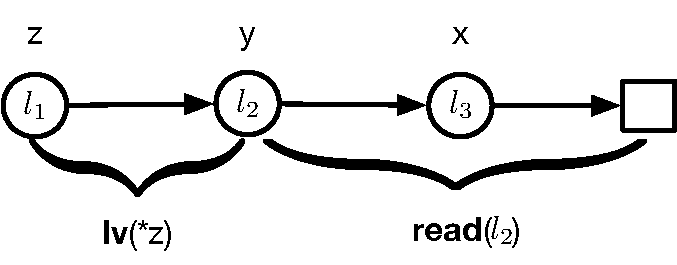
\includegraphics[scale=0.4]{dereferencedemo}
%	\end{center}
%	\vspace{-0.5cm}
%	\caption{An example of dereference}
%	\label{fig:deferencedemo}
%\end{minipage}
%	\vspace{-0.6cm}
%\end{figure*}



%\RuleEnv{Read-Ref\label{Read-shrRef}}{
%$l\mapsto_{lf(l_b,l_e)} \terminal{shrRef}(l')\in S$\quad$l''=current\_Loc$\\
%$S'=S\biguplus (l\mapsto_{lf(l_b,l'')}\terminal{shrRef}(l'))$\quad
%$\nexists l_1\mapsto_{e(l_2)} \terminal{mutRef}(l')\in S,\terminal{lc}(l,l'',l_1,l_2)$\\
%$\cfg{S',\terminal{read}(l')}\rightarrow\cfg{S'',rs(\_)}$\\
%\hline
%$\cfg{S,* * e}\rightarrow\cfg{S', v}$
%}

%\RuleEnv{Read-Ref\label{Read-mutRef}}{
%	$l\mapsto_{e(\_)} \terminal{shrRef}(l')\in S$\quad$l''=current\_Loc$\\
%	$S'=S\biguplus (l\mapsto_{e(l'')}\terminal{shrRef}(l'))$\quad
%	$\nexists l_1\mapsto_{e(l_2)} \terminal{mutRef}(l')\in S,\terminal{lc}(l,l'',l_1,l_2)$\\
%	$\nexists l_1\mapsto_{e(l_2)} \terminal{shrRef}(l')\in S,\terminal{lc}(l,l'',l_1,l_2)$\quad
%	$\cfg{S',\terminal{read}(l')}\rightarrow\cfg{S'',rs(\_)}$\\
%	\hline
%	$\cfg{S,\terminal{read}(l)}\rightarrow \cfg{S'',\terminal{shrRef}(l')}$
%}






%\TwoColumn{
%\ruleEnv{Dereference-Imm-Ref}{
%$\langle C, \terminal{lv}(e)\rangle\rightarrow \langle C, l\rangle$\\
%\hline 
%$\cfg{C, \terminal{* shrRef}(e)}\rightarrow \cfg{C, l}$
%}
%}{
%\ruleEnv{Dereference-Mut-Ref}{
%	$\cfg{ C, \terminal{lv}(e)} \rightarrow\cfg{C, l}$\\
%	\hline 
%$\cfg{C, \terminal{* mutRef} (e)}\rightarrow \cfg{C,l}$
%}
%}

%\TwoColumn{
%\ruleEnv{Read-Var}{
%	$(x\mapsto l\in E)$\quad $(l\mapsto v\in S)\quad v\neq \bot$\\
%	$\nexists~l', l'\mapsto \terminal{mutRef}(l)\in S$\\
%	\hline
%	$\cfg{C,\terminal{read(x)}}\rightarrow\cfg{C,v}$
%}~~
%}
%{
%\ruleEnv{Dereference-Deref}{
%	$ x\mapsto i\in E\quad i\mapsto v\in S \quad v\neq \terminal{uninit}$\\
%	\hline 
%	$\cfg{C, \terminal{*}x}\rightarrow \cfg{C, v}$
%}}
%
%


%	\RuleEnv{Dereference-Field}{
%		$x.i\mapsto v\in E\quad v\neq\terminal{
%		uninit}$\\
%		\hline
%		$(C, \terminal{*} x.i)\rightarrow (C,v)$
%	}


%\RuleEnv{Dereference-Ref}{
%$\cfg{C, \terminal{*} e}\rightarrow \cfg{C', e'}$\quad$\cfg{C', * e'}\rightarrow\cfg{C'', e''}$\\
%\hline
%$\cfg{C, \terminal{*} \terminal{*} e}\rightarrow \cfg{C'', e''}$
%}








%\TwoColumn{
%\ruleEnv{LValue-Var}{
%$x\mapsto l\in E$\\
%\hline
%$\cfg{C,\terminal{lv}(x)}\rightarrow\cfg{C,l}$
%}
%}{
%\ruleEnv{LValue-Deref}{
%	$\cfg{C,\terminal{\terminal{lv}(e)}}\rightarrow\cfg{C',l}$\quad$l\mapsto l'\in S$\\
%	\hline
%	$\cfg{C, \terminal{lv}(* e)}\rightarrow\cfg{C',l'}$
%}}

\paragraph{$(6)$ Transferring.}

We have $5$ semantics rules for transferring. Rule \refrule{Transfer-Resource} transfers a newly allocated resource to a variable. It just updates the value of the location $l$ with the new resource in the cell $S$.

Rule \refrule{Transfer-Move} moves a resource owned by an expression $e$ to the lvalue of an expression $e'$.
It first computes the lvalue of $e$, which is a location $l$ pointing to a non-copyable resource.
Therefore the location $l$ has to be uninitialized due to the move operation, and
the lvalue of  $e'$ is the location $l'$ that now has the ownership of the resource.
Rule \refrule{Transfer-Move} also requires that there are not other references to the location $l$,
which is checked by $\nexists l_n\mapsto_{lf(t_b,t_e)}\terminal{anyRef}(l),t_e\geq t_c$.
The symbol \terminal{anyRef} denotes \terminal{shrRef} or \terminal{mutRef}.
The premise $W'''=W''\cup\{write(\terminal{wv}(e',E''),t_c)\}$ records the
writing operation for the written location (denoted as \terminal{wv}$(e',E'')$) at the current time. 
The calculation for \terminal{wv} is as follows: 
\[
\terminal{wv}(x,E'')=E''(x)\quad\quad\terminal{wv}(*x,E'')=\terminal{wv}(x,E'')\quad\quad\terminal{wv}(x.i,E'')=E''(x).1
\]
Rule \refrule{Transfer-Copy} is similar to \refrule{Transfer-Move} except that the location of  $e$ points to a resource that is copyable and therefore it is not necessary to uninitialize $l$.

Rule \refrule{Transfer-shrRef} transfers a shared reference to a variable.
The lvalue of $e$ is a location that stores a shared reference.
The transferring semantics assigns the location $l'$ with $(t_c,t_c,\terminal{shrRef}(l_1))$,
which 
means that a new shared reference to $l_1$ is created with the lifetime from $t_c$ to $t_c$.
Rule \refrule{Transfer-mutRef} is similar to \refrule{Transfer-shrRef} except that we also need to 
move the mutable reference from the location $l$ to $l'$ and check whether $l$ has been borrowed or not, i.e. whether there are some references to it.



\RuleEnvShort{Transfer-Resource\label{Transfer-Resource}}{
	$C=(E,S,W)$\quad
$x\mapsto l\in E$\quad $S'=S\biguplus(l\rightarrow \terminal{rs}(r))$\quad $Timer+$\\
\hline
$\langle C,\terminal{transfer}~\terminal{rs}(r)\, x\rangle\rightarrow (E,S',W)$
}


\RuleEnv{Transfer-Move\label{Transfer-Move}}{
$\cfg{C,\terminal{lv}(e)}\rightarrow^+ \cfg{C',l}$\quad$C'=(E',S',W')$\quad$l\mapsto \terminal{rs}(ps)\in S'$\quad$copy\notin ps$ \\
$\cfg{C', \terminal{lv}(e')}\rightarrow \cfg{C'',l'}$\quad$C''=(E'',S'',W'')$\quad$S'''=S''\biguplus (l'\mapsto \terminal{rs}(k))\biguplus (l\mapsto\bot)$\\
$t_c=Timer+$\quad
$\nexists l_n\mapsto_{lf(t_b,t_e)}\terminal{anyRef}(l),t_e\geq t_c$\quad$W'''=W''\cup\{write(\terminal{wv}(e',E''),t_c)\}$\\
\hline
$\cfg{C, \terminal{transfer}\,e, e'}\rightarrow (E'',S''',W''')$
}


\RuleEnvShort{Transfer-Copy\label{Transfer-Copy}}{
$\cfg{C,\terminal{lv}(e)}\rightarrow^+ \cfg{C',l}$\quad$C'=(E',S',W')$\quad$l\mapsto \terminal{rs}(ps)\in S'$\quad$copy\in ps$ \\
$Timer+$\quad
$\cfg{C',  \terminal{lv}(e')}\rightarrow \cfg{C'',l'}$\quad$C''=(E'',S'',W'')$\\$S'''=S''\biguplus (l'\mapsto \terminal{rs}(k))$\quad$W'''=W''\cup\{write(\terminal{wv}(e',E''),t_c)\}$\\
\hline
$\cfg{C, \terminal{transfer}\,e, e'}\rightarrow (E'',S''',W''')$
}

\RuleEnv{Transfer-shrRef\label{Transfer-shrRef}}{
	$\cfg{C,\terminal{lv}(e)}\rightarrow \cfg{C',l}$\quad$l\mapsto_{lf(\_,\_)} \terminal{shrRef}(l_1)\in S$\quad$t_c=Timer+$\quad$C''=(E'',S'',W'')$\\
	$\cfg{C',  \terminal{lv}(e')}\rightarrow \cfg{C'',l'}$\quad$S'''=S''\biguplus (l'\mapsto_{lf(t_c,t_c)} \terminal{shrRef}(l_1))$\\$W'''=W''\cup\{write(\terminal{wv}(e',E''),t_c)\}$\\
	\hline
	$\cfg{C, \terminal{transfer}\,e, e'}\rightarrow (E'',S''',W''')$
}

\RuleEnv{Transfer-mutRef\label{Transfer-mutRef}}{
	$\cfg{C,\terminal{lv}(e)}\rightarrow \cfg{C',l}$\quad$l\mapsto_{lf(\_,\_)} \terminal{mutRef}(l_1)\in S$\quad $C''=(E'',S'',W'')$\quad$t_c=Timer+$\\
	$\cfg{C',  \terminal{lv}(e')}\rightarrow \cfg{C'',l'}$\quad$S'''=S''\biguplus (l'\mapsto_{lf(t_c,t_c)} \terminal{mutRef}(l_1))\biguplus (l\mapsto \bot)$\\
	$\nexists l_n\mapsto_{lf(t_b,t_e)}\terminal{anyRef}(l),t_e\geq t_c$\quad$W'''=W''\cup\{write(\terminal{wv}(e',E''),t_c)\}$\\
	\hline
	$\cfg{C, \terminal{transfer}\,e, e'}\rightarrow (E'',S''',W''')$
}


%\createlinenumber{1}{t1}
%\createlinenumber{2}{t2}
%\createlinenumber{3}{t3}
%\createlinenumber{4}{t4}
%\createlinenumber{5}{}
%\createlinenumber{6}{t5}
\begin{figure}
	\vspace{-0.5cm}
\begin{lstlisting}[escapeinside={(*}{*)}]
decl x;                    -(*$Timer=0, E=\{x\mapsto 0\}, S=\{0\mapsto \bot\},W=\{\}$*)
decl y;	                   -(*$Timer=1, E=\{x\mapsto 0,y\mapsto 1\}, S=\{0\mapsto \bot,1\mapsto \bot\},W=\{\}$*)
transfer newResource() x;  -(*$Timer=2, E=\{x\mapsto 0,y\mapsto 1\}, S=\{0\mapsto \terminal{rs}(),1\mapsto \bot\}$*) 	 
                                      (*$W=\{write(0,2)\}$*)
y borrow x;           -(*$Timer=3, E=\{x\mapsto 0,y\mapsto 1\}, $*)
                         (*$S=\{0\mapsto \terminal{rs}(),1\mapsto_{lf(3,3)}\terminal{shrRef}(0)\},W=\{write(0,2)\}$*)
decl z;               -(*$Timer=4, E=\{x\mapsto 0,y\mapsto 1,z\mapsto 2\},$*) 
                         (*$S=\{0\mapsto \terminal{rs}(),1\mapsto_{lf(3,3)}\terminal{shrRef}(0), 2\mapsto\bot\},W=\{write(0,2)\}$*)
z mborrow x;          -(*$Timer=5, E=\{x\mapsto 0,y\mapsto 1,z\mapsto 2\},W=\{write(0,2)\},$*) 
                         (*$S=\{0\mapsto \terminal{rs}(),1\mapsto_{lf(3,3)}\terminal{shrRef}(0)\},2\mapsto_{lf(5,5)}\terminal{mutRef}(0)\}$*)
y;                    -(*$Timer=6, E=\{x\mapsto 0,y\mapsto 1,z\mapsto 2\},W=\{write(0,2)\}$*) 
                          (*$S=\{0\mapsto \terminal{rs}(),1\mapsto_{lf(3,6)}\terminal{shrRef}(0)\}, 2\mapsto_{lf(5,5)}\terminal{mutRef}(0)\}$*)
\end{lstlisting}
\caption{An example to illustrate the semantics}
\label{fig:exampleborrow}
\vspace{-0.5cm}
\end{figure}

Fig. \ref{fig:exampleborrow} shows an example to illustrate the semantics.
Line 1 creates a new variable \codec{x}, whose newly allocated location is $0$ and is initialized to $\bot$.
Line 3 transfers a non-copyable resource to \codec{x}. The set $W$ is modified with a new element $write(0,2)$, i.e.,
a writing operation is carried out on the location $0$, which is the location of \codec{x} at the time instant $2$.
Line 5 creates a shared reference to \codec{x}, with the lifetime from $3$ to $3$.
Line 9 creates a mutable reference to \codec{x}, with the lifetime from $5$ to $5$.
Line 11 reads the variable \codec{y}, which extends the lifetime of the reference assigned to \codec{y}, i.e., the initial
lifetime is from 3 to 3 and the new lifetime is from 3 to 6.
Therefore an error is detected by Rule \refrule{Read-shrRef}, since the intersection of the lifetimes for the shared reference assigned to \codec{y} and the mutable reference assigned to \codec{z} is not empty. %safe space...that is straightforward , i.e, the intersection of $lf(3,6)$ and $lf(5,5)$ is not empty.



%\createlinenumber{1}{1}
%\createlinenumber{2}{2}
%\createlinenumber{3}{3}
%\createlinenumber{4}{4}
%\createlinenumber{5}{5}
%\createlinenumber{6}{6}

\paragraph{$(7)$ Branches. }
Rule \refrule{Branch} defines the semantics for branches, which non-deterministically selects one branch to execute. 
A new configuration is obtained
by selecting a branch in $B_1,\ldots,B_n$ to execute with the configuration $C$.
%



\TwoColumn{
\ruleEnvS{Branch\label{Branch}}{
	$\exists i, 1\leq i \leq n, \cfg{C,B_i}\rightarrow C'$\\
	\hline
	$\cfg{C, @ B_1,\ldots,B_n}\rightarrow C'$ 
}
}{
\quad
\ruleEnvS{Destruct\label{Destruct}}{$C=(E,S,W)$\quad
	$l\mapsto v\in S$\quad$S'=S\backslash(l\mapsto v)$\\
	\hline
	$\cfg{C, \terminal{destruct}~l ;}\rightarrow (E,S',W)$
}
}





%\TwoColumn{
%\ruleEnv{Non-Determinism\label{Non-Determinism}}{
%$CS'=\{C'\mid \}\exists i, 1\leq i \leq n, \cfg{C, B_i}\rightarrow^+ C'$\\
%\hline
%$\cfg{CS, @ B_1,\ldots,B_n}\rightarrow CS'$ 
%}
%\quad\quad\quad
%}{
%\ruleEnv{Repeat-Success}{
%$\cfg{C,B}\rightarrow C'$\quad$\cfg{C', B}\rightarrow C''$\\
%\hline 
%$\cfg{C',\terminal{!} B}\rightarrow C''$
%}}
%
%\TwoColumn{
%\ruleEnv{Repeat-Break1}{
%$\cfg{C,B}\rightarrow \cfg{C',\terminal{break}~ ...}$\\
%\hline
%$(C, \terminal{!} B)\rightarrow C'$
%}
%}{
%\ruleEnv{Repeat-Break2}{
%$\cfg{C,B}\rightarrow C'$\quad $(C',B)\rightarrow \cfg{C'',\terminal{break}~ ...}$\\
%\hline
%$(C, \terminal{!} B)\rightarrow C''$
%}}
%
%
%
%\RuleEnv{Repeat-continue-Break1}{
%		$\cfg{C,B}\rightarrow \cfg{C',\terminal{continue}~ ...}$\quad $(C',B)\rightarrow \cfg{C'',\terminal{break}~ ...}$\\
%		\hline
%		$(C, \terminal{!} B)\rightarrow C'$
%}
%
%\RuleEnv{Repeat-continue1}{
%	$\cfg{C,B}\rightarrow C'$\quad $(C',B)\rightarrow \cfg{C'',\terminal{continue}~ ...}$\\
%	\hline
%	$(C, \terminal{!} B)\rightarrow C''$
%}
%
%
%\RuleEnv{Repeat-continue1}{
%	$\cfg{C,B}\rightarrow \cfg{C',\terminal{continue}}$\quad $(C',B)\rightarrow \cfg{C'',\terminal{continue}~ ...}$\\
%	\hline
%	$(C, \terminal{!} B)\rightarrow C''$
%}
%
%\RuleEnv{Repeat-continue2}{
%	$\cfg{C,B}\rightarrow \cfg{C',\terminal{continue}}$\quad $(C',B)\rightarrow C''$\\
%	\hline
%	$(C, \terminal{!} B)\rightarrow C''$
%}
%
%\RuleEnv{Destruct-Deallocate}{
%	$x\mapsto l \in E$\quad$l\mapsto \terminal{rs}(r)\in S$\quad$\nexists l',l'\mapsto \terminal{rs}(r)\in S\land l\neq l'$\quad$\cfg{C,\terminal{deallocate}~\terminal{rs}(k)}\rightarrow C'$\\
%\hline
%$\cfg{C, \terminal{destruct}~x ;}\rightarrow C'$
%}

%\RuleEnv{Destruct-Idle}{
%	$x\mapsto i \in E$\quad$i\mapsto \terminal{rs}(k)\in S$\quad$\exists j,j\mapsto \terminal{rs}(k)\in S\land j\neq i$\\
%	\hline
%	$\cfg{C, \terminal{destruct}~x ;}\rightarrow C$
%}

\paragraph{$(8)$ Destruct, Block, Sequential.}
Rule \refrule{Destruct} defines the semantics of destructing a location in the cell $S$.
Rule \refrule{Block} defines the semantics for a \emph{block}.
The domain for a map $M$ is defined as  $domain(M)\triangleq\{x\mid \exists v,x\mapsto v\in M \}$.
The semantics of blocks includes: (1) executing the body of the block and (2) restoring the cell $E$ and $S$, since the local variables are only available within the block. 
Rule \refrule{Sequential} defines the semantics for sequential composition and its semantics is intuitive.

\TwoColumn{
\ruleEnvS{Block\label{Block}}{
	$C=(E,S,W)$\quad$\cfg{C,ss}\rightarrow C'$\quad$C'=(E',S',W')$\\
$domain(S')\backslash domain(S)=\{l_1,\ldots,l_k\}$\\
$\cfg{C',\terminal{destruct}(l_1);\ldots ;\terminal{destruct}(l_k)}\rightarrow (E'',S'',W'')$\\
\hline
$\cfg{C, \{ ss \}}\rightarrow (E,S'',W'')$
}
}{
\ruleEnv{Sequential\label{Sequential}}{
	$\cfg{C,s_1}\rightarrow C'$\quad$\cfg{C',s_2}\rightarrow C''$\\
	\hline
	$\cfg{C, s_1~s_2}\rightarrow C''$
}
}

%\RuleEnv{Release}{
%$S'=\{\terminal{block}(\terminal{shrRef}(\_),i),\terminal{block}(\terminal{mutRef}(\_),i)\}$\quad $S_1=S$\quad
%$domain(S,S')=\{i_1,\ldots,i_n\}$\\
%$\forall  2\leq k \leq n, S_k=
%\left\{\begin{matrix}
%S_{k-1}\biguplus (i_{k-1}\mapsto \terminal{shrRef}(j)) & i_{k-1}
%\mapsto \terminal{block}(\terminal{shrRef}(j))\in S \\ 
%S_{k-1}\biguplus (i_{k-1}\mapsto \terminal{mutRef}(j)) & i_{k-1}
%\mapsto \terminal{block}(\terminal{mutRef}(j))\in S 
%\end{matrix}\right.$
%\\
%\hline
%$\cfg{S, \terminal{release}~i ;}\rightarrow S_k$}



\paragraph{$(9)$ Function Calls.} Rule \refrule{Call} defines the semantics of function calls. It translates a function call to a block $\{\terminal{transfer}\,e_1\,p_1 \terminal{;}\ldots\terminal{; } \terminal{transfer}\,e_n\, p_n\terminal{;}~B\}$, where
$\terminal{transfer}~e_i~p_i$ transfers the argument $e_i$ to the parameter $p_i$. The body $B$ is executed after assigning arguments to parameters.
OSL only supports non-recursive functions.
Unlike loop (The rule for loop will be introduced later), function calls need to consider stack, which makes it hard to compute the fix set of configurations, since the stack keeps increases.
 It does not mean OSL cannot check
recursive functions in other languages.
In fact, in many cases, recursive functions in other languages, such as Rust, can
be translated into non-recursive functions in OSL, especially when the input parameters
and return value has no relations w.r.t lifetimes. Appendix \ref{appendix:recursiveexample} gives an example.

% Note that, in OSL, we do not use recursive functions since we abstract 
%the relations between variables. %{\color{red} this assume it also applies to loops?}.
%Recursive functions in Rust can be translated into non-recursive functions in OSL. 
%For some examples, the translation need to perform over-approximation. %{\color{red} what does this exactly mean?}.

\TwoColumn{
\ruleEnv{Call\label{Call}}{
	$\terminal{fn } f (x_1:t_1,\ldots,x_n:t_n)\rightarrow t~B$\quad$ $\\
	$\cfg{C,\{\terminal{transfer}\,e_1\,p_1 \terminal{;}\ldots \terminal{transfer}\,e_n\, p_n\terminal{;}~B\}}$\\$\rightarrow\cfg{C',v}$\\
	\hline
	$\cfg{C, \terminal{call}\,f\,(e_1,\ldots,e_n)}\rightarrow\cfg{C',v}$
}}{\quad\quad
\ruleEnv{Set\label{Set}}{
		$\forall C\in CS. \exists C'. \cfg{C,CT}\rightarrow C'$ \\
	$CS'=\{C'\mid \exists C\in CS, \cfg{C,CT}\rightarrow C'\}$\\
	\hline
	$\cfg{CS,CT}\rightarrow_c CS'$
}}

\subsection{Semantics for a set of configurations}
To introduce the semantics for loops it is necessary first to introduce the semantics for a set of configurations.
%
Consider a set $CS$ of configurations and a statement $CT$ in OSL, which is not the loop construct. The semantics of the execution of $CT$ under $CS$ is defined in Rule \refrule{Set}.



Rule \refrule{Set} defines the semantics for a statement  $CT$ with respect to
 a set of configurations $CS$. 
 This rule requires that $CT$ can be executed under all configurations in $CS$.
 The set $CS'$ is exactly the set of configurations that can be obtained by executing $CT$ under all configurations in $CS$.
% The rule transits to a new set of configurations
%  consisting of the configuration $C'$ such that for any $C$ in $CS$ $<C,CT>$ transits to $C'$, whenever there is not an initial configuration $C$ such that $<C,CS>$ gets stuck.
 
Rule \refrule{Loop} computes the fix set of configurations  from an initial set $CS_0$ of configurations by repeating executing the block $B$ to obtain the configuration of the next iteration. When $CS_i\cong CS_{i+1}$ the fix set of configurations is reached, where $\cong$ is an equivalent relation between two sets of configurations defined as:
\[
CS\cong CS'\triangleq \text{there is a bijection:} f: CS \rightarrow CS' \text{ such that }
\forall C\in CS, C\cong f(C).
\]
The equivalent relation  for two configurations $C=(E,S,W)$ and $C=(E',S',W')$ is defined as:
\[
C\cong C'\triangleq E=E' \land \text{there exists a bijection:} g: S \rightarrow S' \text{ such that }
\]\[
\forall l\mapsto v\in S, g(l\mapsto v)= \begin{cases}
l\mapsto v & v = \terminal{rs}(ps) \text{ or }\bot \\
l\mapsto_{lf(l_b,l_e)\terminal{shrRef}(l)} & v = (\_,\_,\terminal{shrRef}(l))\\
l\mapsto_{lf(l_b,l_e)\terminal{mutRef}(l)} & v = (\_,\_,\terminal{mutRef}(l))\\
\end{cases}
\]

The equivalent relation for the configurations means that the same location in both $S$ and $S'$ points to the same value.
When the locations store references, the lifetimes of in both $S$ and $S'$ can be different.
The symbol `\_' means any value.




\RuleEnvShort{Loop\label{Loop}}{
	$\exists CS_0, CS_1,\ldots, CS_n,$\quad\quad\quad\quad\quad\quad\quad\quad\quad\quad\quad\quad\quad\quad\quad\quad\quad\quad\quad\quad\quad\quad\\ $(CS_0=CS)\land (\cfg{CS_i, B}\rightarrow_c CS_{i+1})\land (CS_n\cong CS_{n-1})$\\
	\hline 
	$\cfg{CS, !B}\rightarrow_c CS_n$
}

There exist pairs $\cfg{CS,P}$, where $CS$ is a set of configurations and $P$ is 
an OSL statement, such that no semantics rule matches it.
Then this is an illegal pair for which the execution of the semantics gets stuck, uncovering unsafe memory risks.
%
We now define the notion of safe programs in OSL.

\begin{definition}[Safe Programs]
	For an OSL program fragment $P$, and a set $CS$ of configurations,
	if there exists another set  $CS'$ of configurations, such that $\cfg{CS,P}\rightarrow_c CS'$ then
	we say that $P$ is a \textbf{safe program} with respect to $CS$.
\end{definition}

%For each OSL function, it can be verified with the semantics by (1) constructing a value for each input parameter and then calling the function.
%Fig. \ref{fig:voslfunctions} shows an example.
%On the left, it is a function \codec{g} with three parameters,
%where \codec{x} is a variable of a copyable owner type,
%\codec{y} is a variable of a non-copyable owner type,
%\codec{z} is a variable of reference to a non-copyable owner type.
%On the right, three values are created and the function \codec{g} is called with the three values.
%The reason why an OSL function can be verified like this is that
%we abstract the values in Rust with only two types.
%
%\begin{figure}
%\centering
%\begin{tabular}{rcl}
%\begin{minipage}{0.4\textwidth}
%\renewcommand{\ttdefault}{pcr}
%\begin{lstlisting}
%fn g(x:own(copy),y:own(),
%       z:ref(own()))
%	   -> own() { ... }
%\end{lstlisting}
%\end{minipage}
%& \quad\quad\quad\quad &
%\begin{minipage}{0.4\textwidth}
%	\renewcommand{\ttdefault}{pcr}
%	\begin{lstlisting}
%decl x; transfer new_resource x;
%decl y; transfer new_resource y;
%decl zt; transfer new_resource z;
%decl z; z borrow zt;
%call g (x,y,z)
%	\end{lstlisting}
%\end{minipage}
%\end{tabular}
%\caption{An example of verifying OSL functions}
%\label{fig:voslfunctions}
%\end{figure}

\subsection{Extending the Semantics to Fields}

In Rust, we can not only move or borrow a variable, but also move or borrow a field of
a variable. In order to also supports this, we introduce another kind of locations.
For a variable $x$, whose location is $l$, one of its fields can be $l.2$, which denotes the
second field of $l$.
The following example shows this case.

\begin{tabular}{rcl}
\begin{minipage}{0.33\textwidth}
\renewcommand{\ttdefault}{pcr}
\begin{lstlisting}
let p = Point {x:1,y:2};
let b1 = & mut p.x;
let b2 = & mut p.y;
\end{lstlisting}
\end{minipage}
& \quad\quad $\Rightarrow$ \quad\quad\quad &
\begin{minipage}{0.4\textwidth}
	\renewcommand{\ttdefault}{pcr}
	\begin{lstlisting}
decl p; transfer new_resource p;
decl b1; b1 mborrow p.0;
decl b2; b2 mborrow p.1;
	\end{lstlisting}
\end{minipage}

\end{tabular}


\section{Properties of Semantics}
\label{sec:properties}

In this section, we discuss the properties of the semantics to show that OSL is capable of detecting memory unsafe risks.
The proofs of the theorems are shown in Appendix  \ref{appendix:proofidea}.

The first one is the termination of the execution. Theorem \ref{thm:terminal} shows that the execution of an OSL program always terminates, i.e., the memory safety checking is always terminated. There are two cases for the termination: the program is a safe program or the program gets stuck at the middle of the execution. 

\begin{theorem}[Termination]
	\label{thm:terminal}
	For an OSL program $P$, the execution of $P$ with the initial set $CS$ of configurations is always terminated.
\end{theorem}

\begin{definition}[States]
 A state of OSL is defined a  3-tuple $(C, P, t)$, where $C$ is a configuration, $P$ is program fragment to be executed under the configuration $C$ at the time instant $t$.
\end{definition}

\begin{definition}[Reachable States]
	\label{def:reachablestates}
For a configuration $C$,  a time instant $t$, and an OSL program $P$, the set of reachable states from $(C,P,t)$ contains 
all the intermediate states generated by the semantics rules $\rightarrow$ during the execution starting from $\cfg{C,P}$ with $t$ as the initial time. 
The relation that a state $(C',P',t')$ is reachable from $(C,P,t)$ is denoted as $(C,P,t)\rightsquigarrow(C',P',t').$
\end{definition}

Definition \ref{def:reachablestates} defines the notion of reachable states. Theorem \ref{lemma:no-dangling-pointers}  specifies that no reachable state contains dangling pointers, i.e.,
during the lifetime of a reference, the referent should be always valid.
Theorem \ref{thm:no-data-races} specifies that no reachable state contains data races, i.e.,
the intersection of the lifetimes of two references should be empty.



\begin{theorem}[No Dangling Pointers]
	\label{lemma:no-dangling-pointers}
For an OSL program $P$ and a time instant $t$, for all reachable states $(C',P',t')$ from $((\emptyset,\emptyset,\emptyset),P,t)$ where $C'=(E',S',W')$, it satisfies that 
$\forall l\mapsto_{lf(t_b,t_e)} \terminal{anyRef}(l')\in S', \nexists ((E'',S'',W''),P'',t''),$ $ ((\emptyset,\emptyset,\emptyset),P,t)\rightsquigarrow((E'',S'',W''),P'',t'')\land t_b\leq t''\leq t_e\land(l'\mapsto\bot)\in S''$.

\end{theorem}



\begin{theorem}[No Data Races]
	\label{thm:no-data-races}
For an OSL program $P$ and a time instant $t$, for all reachable states $(C',P',t')$ from $(\{(\emptyset,\emptyset,\emptyset)\},P,t)$ where $C'=(E',S',W')$, it satisfies that $\forall l_1\in Loc, l_2\in Loc,  l_1\mapsto_{lf(l_b,l_e)} \terminal{anyRef}(l)\in S'\land l_2\mapsto_{lf(l_b',l_e')}\terminal{mutRef}(l)\in S'\rightarrow\neg \terminal{lc}(l_b,l_e,l_b',l_e')\land \neg \terminal{lc}(l_b',l_e',l_b,l_e).$
\end{theorem} 





\section{Implementation and Evaluation}
\label{sec:imp-eval}


The semantics of OSL has been implemented in K-Framework with around 200 syntax and semantics rules. It can be downloaded at \cite{OSL}.
The executable semantics tool generated by $\mathbb{K}$ is called K-OSL.
For an OSL program, K-OSL executes the program with the semantics of OSL.
If the program is not a safe program then K-OSL will show the intermediate configurations and program fragments that 
lead to the memory unsafe risks.
%K-OSL is efficient since the domain of values is limited and the semantics is sequential.




One of the objectives for OSL is the application to other languages by defining translations from the languages to OSL.
In this section, we discuss the way of reusing OSL for C.
The challenge is that in Rust, we explicitly label each variable and
each reference as mutable or not.
But in C, we do not have such information.
There are two ways to solve this: (1) add the mutable information to comments for
statements, 
%
(2) design an automatic way to decide the mutable information of variables and references.

%\begin{center}
%\begin{minipage}{0.7\textwidth}
%	\vspace{-0.5cm}
%	\renewcommand{\ttdefault}{pcr}
%\begin{lstlisting}[caption={An example of C program with comments}\label{lst:osl2c}]
%int *x;    //x is mutable
%x = (int*) malloc(sizeof(int));
%int **y;   //y is immutable
%y = & x;   //& x is a mutable reference
%\end{lstlisting}
%\vspace{-0.5cm}
%\end{minipage}
%\end{center}
%
%Listing \ref{lst:osl2c} is an example to show the correspondence between C and OSL.
%Line 1 is the declaration of a variable \codec{x} of the type \codec{int *},
%which is a pointer to an address in the heap.
%Line 2 allocates a block for \codec{x} and we can view that \codec{x} has the ownership of the block.
%Line 3 is the declaration of the pointer of the pointer to an integer.
%Line 4 assigns the address of \codec{x} to \codec{y}
%and we can view it as a reference to \codec{x}, i.e., \codec{y} borrows \codec{x}.
%The comments in the Listing explicitly express that \codec{x} is mutable, \codec{y} is imutable,  \codec{\& x} is mutable reference.
%If we select the first way, the translation needs to read the comments to extract the information for variables and references.

Here, we give an example to automatically decide the mutable information for variables and references.

\begin{enumerate}
	\item all variables are mutable, therefore a mutable reference to any variable is feasible, 
	\item dynamic allocated blocks are new resources without the \terminal{copy} property,
	\item a variable that points the address of a newly allocated block in the heap has the ownership of the resource,
	\item values of scalar types, such as int and char, and values allocated in the stack except pointers are resources with the \terminal{copy} property,
	\item ampersand operator ``\codec{\&}", which denotes the address of a variable, creates references,
	\item a reference is mutable if there exists a writing to the referent of the reference, and the writing is carried out though the reference.
\end{enumerate}

This set of rules are not enough to deal with the full set of C language, but it is enough to show the usefulness of OSL.
Rule 6 needs to scan the code that the reference is valid to decide it.
Fig. \ref{fig:translation1} shows an example of detecting dangling pointers in C by using OSL.
The variable \codec{ptr} is a dangling pointer after line 5, since \codec{x} is invalid.
The corresponding OSL code is on the right, which is not accepted by the semantics of OSL, since
 line 6 reads the dangling pointer. 

\begin{figure}
		\vspace{-0.5cm}
\begin{center}
\begin{tabular}{ccc}
\begin{minipage}{0.25\textwidth}
\renewcommand{\ttdefault}{pcr}
\begin{lstlisting}[language=C]
int *ptr;
{
   int x = 5;
   ptr = & x;
}
printf("%d", *ptr );
\end{lstlisting}
\end{minipage}
 & \quad$\Rightarrow$\quad \quad\quad& 
 \begin{minipage}{0.5\textwidth}
 	\renewcommand{\ttdefault}{pcr}{\footnotesize
 	\begin{lstlisting}
decl ptr;
{
  decl x; transfer (new_resource copy) x;
  ptr borrow x;
}
* ptr;
 \end{lstlisting}}
 \end{minipage} 
\end{tabular}
\end{center}
\vspace{-0.5cm}
\caption{Translation 1}
\vspace{-0.5cm}
\label{fig:translation1}
\end{figure}

Fig. \ref{fig:translation2} shows an example of move semantics in C.
At line 5 on the left, the C program creates a variable and assigning
a value of the type \codec{Point} to it.
Since this value is located in the stack, it is a copyable resource.
After executing line 6, the variable \codec{p1} still holds the ownership of its resource and
therefore Line 7 is legal.
At line 8 of the C code, it creates a new block in the heap and assigns to \codec{p3}.
The memory block is not copyable.
Line 10 in the C code transfers the ownership of the resource from \codec{p3} to \codec{p4}.
After that, \codec{p3} does not hold the ownership of the resource.
Therefore line 11 in the C code is illegal.
After translating it to OSL code, our semantics can detect it.

\begin{figure}
	\vspace{-0.5cm}
\begin{tabular}{ccc}
	\begin{minipage}{0.45\textwidth}
		\renewcommand{\ttdefault}{pcr}
		\begin{lstlisting}[language=C]
struct Point {
 int x, y;
};
--------------------------
struct Point p1 = {0,1};
struct Point p2 = p1 ;
printf("%d", p1);
struct Point * p3 = (struct Point *) 
       malloc (sizeof(struct Point));
struct Point * p4 = p3;
struct Point * p5 = p3
		\end{lstlisting}
	\end{minipage}
	& \quad$\Rightarrow$\quad \quad~& 
	\begin{minipage}{0.38\textwidth}
		\renewcommand{\ttdefault}{pcr}{\scriptsize
			\begin{lstlisting}
decl p1; 
transfer (new_resource copy) p1;
decl p2; 
transfer p1 p2;
* p1;
decl p3; 
transfer new_resource p3;
decl p4; 
transfer p3 p4;
decl p5; 
transfer p3 p5;
			\end{lstlisting}}
	\end{minipage} 
\end{tabular}
\caption{Translation 2}
\label{fig:translation2}
\vspace{-0.5cm}
\end{figure}
Fig. \ref{fig:translation3} shows a data race in the C code with respect to OSL semantics.
Both variables \codec{b} and \codec{c} borrow the variable \codec{a}, but
the variable \codec{b} mutably borrows the variable \codec{a}, since there is
a writing operation through \codec{b} at line 7.
The corresponding OSL program is also illegal since the lifetime
of \codec{b} includes lines 5-7 and the lifetime of \codec{c} is line 6.
Therefore their intersection is not empty.

\begin{figure}
	\vspace{-0.2cm}
\begin{center}
	\begin{tabular}{ccc}
		\begin{minipage}{0.25\textwidth}
			\renewcommand{\ttdefault}{pcr}
			\begin{lstlisting}[language=C]
int a;
a = 6;
int * b;
int * c;
b = & a;
c = & a;
*b = 7;
	\end{lstlisting}
		\end{minipage}
		& \quad$\Rightarrow$\quad \quad\quad& 
		\begin{minipage}{0.43\textwidth}
			\renewcommand{\ttdefault}{pcr}{\scriptsize
				\begin{lstlisting}
decl a;
transfer (new_resource copy) x;
decl b; 
decl c;
b mborrow a;
c borrow a;
transfer (new_resource copy) (*b);
				\end{lstlisting}}
		\end{minipage} 
	\end{tabular}
\end{center}
\vspace{-0.5cm}
\caption{Translation 3}
\label{fig:translation3}
\vspace{-0.5cm}
\end{figure}

%The 3 translations from C  to OSL  show that the rules for the translation is feasible and
%OSL semantics can be used to detect memory unsafe risks in C.

At last, we introduce the application of OSL for C by a case study.
On the left in Fig. \ref{fig:osltoc}, it is a C program from \cite{DBLP:journals/virology/FeistMP14}.
There is a dangling pointer in the C code.
The main idea is that the function \codec{index\_user} puts \codec{p}, the 
function argument, in the global variable \codec{p\_global}(line 8) and restores the previous value of \codec{p\_global}(just before the end of the function, line 14). But, when the condition \codec{cmp} succeeds at line 9, \codec{index\_user} does not restore the value of \codec{p\_global}.  Therefore, in this case \codec{p\_global} and \codec{p} point to the same resource.
So, if during the call at line 26 this behaviour happens, \codec{p\_global} will point to the same memory area that \codec{p\_index} points to and it will be freed at line 27. Therefore \codec{p\_global} will become a dangling pointer. 

On the right of Fig. \ref{fig:osltoc} is the OSL program translated from the C code.
The dangling pointer can also be detected by K-OSL by the rule: \emph{unique ownership} in OSL.
When calling \codec{index\_user} at line 27 in the OSL code, if \codec{p\_global} is not restored then
\codec{p\_global} has the ownership of the resource moved from \codec{p\_index} and \codec{p\_index} is uninitialized now.
Therefore at line 28, the operation \codec{deallocate(p\_index)} is illegal since \codec{p\_index} is moved and uninitialized.






\begin{figure}[t]
\begin{minipage}{0.5\textwidth}
	\renewcommand{\ttdefault}{pcr}
\begin{lstlisting}[language=C]
int * p_global;
int cmp () { 
  return *p_global>=MIN&&*p_global<=MAX;
} 
void index_user (int * p) {                                                                                                                                                            
  int * p_global_save ; 
  p_global_save = p_global; 
  p_global = p; 
  if ( cmp () <=0) { 
    printf("The secret is 
                   greater than 50\n"); 
    return ; }
  printf("The secret is less than 50\n");
  p_global = p_global_save; 
  return;
}     
int main( int argc , char * argv []) {                                                                                                                                            
 int * p_index ,* p_pass; 
 p_global =( int *) malloc(sizeof(int));
 * p_global = SECRET_PASS ;
 if (atoi(argv[1])==MODE_EASY){ 
   p_index =( int *)malloc(sizeof(int));
   printf("Give a number 
            between 0 and 100\n"); 
   scanf("%d",p_index); 
   index_user ( p_index ) ;
   free (p_index) ; } 
   else { 
       printf ( " Good luck ! \ n " ) ; 
   } 
   p_pass =( int *)malloc(sizeof(int));  
   printf ( " Give the secret \ n " ) ;
   scanf ( " % d " , p_pass ) ;
   if (* p_pass ==* p_global ) { 
       printf ( " Congrats ! \n " ) ; }
    else { printf ( " Sorry ...\n " ) ; } 
   return 0; 
}                               
\end{lstlisting}
\end{minipage}
~~~~~~~~~~
\begin{minipage}{0.43\textwidth}
	\renewcommand{\ttdefault}{pcr}
\begin{lstlisting}
decl p_global ;
fn cmp() -> own(copy) {
  p_global; val(newResource)
}
fn index_user(int *p) {
 decl p_global_save;
 transfer p_global p_global_save;
 transfer p p_global;
 call cmp ();
 @{

 },{
  transfer p_global_save p_global;
 }
}


fn main(arg:own(copy),argv:own()){
 decl p_index; decl p_pass;
 transfer newResource() p_global;
 argv;
 @{
   transfer newResource() p_index;
   
   
   
   call index_user(p_index);
   deallocate(p_index);
 }, {
 
 };
 transfer newResource() p_pass;


 *p_pass;
 *p_global;
 @ {} {}
}
\end{lstlisting}
\end{minipage}
\caption{A case study of OSL to C}
\label{fig:osltoc}
\vspace{-0.5cm}
\end{figure}








\section{Related Work}
\label{sec:relatedwork}

Memory safety and the vulnerabilities follow its absence are common concerns. There are tons of works focusing memory safety.


\textbf{Ensuring memory safety by type systems.} Most works in this category define memory errors as attempts to use a pointer to access a location. Cyclone \cite{DBLP:journals/scp/SwamyHMGJ06} is a language with a type system for safe manual memory management.  SoftBound \cite {DBLP:conf/pldi/NagarakatteZMZ09} is a compile time transformation for enforcing complete spatial safety of C, including the detection of bounds violations within an object. CES \cite{DBLP:conf/iwmm/NagarakatteZMZ10} a compiler pass for preventing temporal safety violations in C programs, including accessing dangling pointers into freed heap regions and stale stack frames. 
Mezzo \cite{DBLP:conf/icfp/PottierP13} and Rust \cite{rusthome} are languages, whose type systems control aliasing and ownership. These two language are able to detect dangling pointers and data races. 


\textbf{Reasoning memory safety by separation logic.}
Separation logic \cite{DBLP:conf/lics/Reynolds02}\cite{DBLP:conf/fossacs/YangO02}  is deeply linked to memory safety.
Amorim et. al. \cite{DBLP:conf/post/AmorimHP18} gave a rigorous characterization of what it means for a programming language to be memory safe based on separation logic. Kaiser et. al. \cite{DBLP:conf/ecoop/KaiserDDLV17} proposed a strong logic for weak memory based separation logic to reason about release-acquire consistency.

\textbf{Reasoning memory safety  by model checking and runtime verification.} Model checking and runtime verification
are two techniques that can be exploited to automatically reasoning memory safety.
Beyer et. al. proposed a method to check memory safety of C programs based on Blast \cite{DBLP:conf/spin/HenzingerJMS03}, which is a C model checker.
Rosu et. al. \cite{DBLP:conf/rv/RosuSS09} proposed a runtime  verification technique for checking the memory safety of C.

Our work is not in the three categories. We aim at providing an intermediate language that can be reused by existing languages for memory safety checking and decoupling the ownership from Rust. OSL is only capable of checking the memory safety properties that can be checked by 
the ownership system.



\section{Conclusion and Future Work}
\label{sec:conclusion}

In this paper, we propose a language called OSL to extract the ownership system from Rust.
The motivations for OSL are: (1) constructing a formalized language independent ownership checker; (2) 
reusing the ownership checking for other languages.
The operational semantics of OSL is in fact the semantics of ownership checking and it is implemented in $\mathbb{K}$.
We also illustrate the application of OSL for C to check memory unsafe risks.
In the future, we plan to implement a ownership checker for the full class of C based on OSL and exploit the application
of OSL to other languages.

\bibliographystyle{plain}
\bibliography{reference.bib}


\appendix
\section{Proof Ideas}
\label{appendix:proofidea}

\paragraph{The proof of Theorem \ref{thm:terminal}.} 
In order to prove the termination of the execution of the semantics, we need to show
that the computation of a loop is always terminated.
As in Rule \refrule{Loop}, a sequence of sets of configurations $CS_0,CS_1,\ldots$ is generated.
We prove that the set of all possible elements in $CS_i$ is finite.
Each element in $CS_i$ is a configuration $(E,S,W)$.
The cell $E$ is fixed since the local variables created in the loop block $B$ are removed
after executing the block. 
The domain of $S$, i.e., the locations of variables, is  fixed since $E$ is fixed.
Therefore the range of values in $S$ determines the number of different configurations.
Since we only have 4 kinds of values. 
(1) The the number of values $\terminal{rs}(ps)$ depends on the number of properties, since the set of properties is finite, therefore this kind of values is finite.
(2) The number of shared and mutable references is dependent on the locations of variables.
Since the number of variables is finite, therefore the number of references is finite.
(3) The symbol $\bot$ is only one value, therefore it is finite.

In conclusion, since the number of values for locations is finite, therefore the number of configurations is finite.




\paragraph{The proof of Theorem \ref{lemma:no-dangling-pointers}.}
In the semantics, only the following 4 rules: \refrule{Read-shrRef}, \refrule{Read-mutRef}, \refrule{LValue-immDref},
\refrule{LValue-mutDref}, extend the lifetime of a reference.
But all these rules check no writing during the lifetime of the reference by $\terminal{wl}$.
The deallocation operation (the semantics of deallocation is not presented in the paper due to page limitation) will also add writing label to the set $W$ in the configuration $(E,S,W)$. Therefore the $\terminal{wl}$ checking in these rules always ensure no reachable state has
 dangling pointers.


\paragraph{The proof of Theorem \ref{thm:no-data-races}.}
As the proof of Theorem \ref{lemma:no-dangling-pointers}, only the following 4 rules: \refrule{Read-shrRef}, \refrule{Read-mutRef}, \refrule{LValue-immDref},
\refrule{LValue-mutDref}, extend the lifetime of a reference.
But all these rules has a premise checking that there no intersection of the lifetime of a reference and the lifetime of a mutable reference by $\terminal{lc}$.
Therefore the semantics ensures no reachable states has data races.

\section{An Example of Recursive Functions in Rust to non-Recursive Functions in OSL}
\label{appendix:recursiveexample}

The recursive Rust function:
\renewcommand{\ttdefault}{pcr}
\begin{lstlisting}
fn sumV(v:&Vec<i32>,i:usize) -> i32 {
   if (i >= v.len()) { 0 }
   else {v[i] + sumV(v,i+1)}
}
\end{lstlisting}

\lstset{
commentstyle=\fontfamily{fve}\selectfont\color{red}, 
}

~\\
The corresponding OSL no-recursive function:
\renewcommand{\ttdefault}{pcr}
\begin{lstlisting}
fn sumV(v: ref('a, own()), i:own(copy)) -> own(copy) {
  //The condition i >= v.len() needs to read both v and i
  i;  v;  //reading for v and i
@ {
  val(newResource(copy))  //This returns the value 0
}, {
  v ; //corresponds to read v[i];
  // the recursive call to sumV(v,i+1) needs not to be carried out since
  // it has no effect on v and i after calling it.
  // We only need to perform the operations for passing v and i 
  // to temporal variables to stimulate the argument passing. 
  decl vt ; transfer v vt;
  i;  //read i for computing i + 1
  decl it; transfer newResource(copy) it;

  val(newResource(copy))  //return a copyable resource
 };
};
\end{lstlisting}

\end{document}


























